\documentclass{article}
\usepackage[utf8]{inputenc}
\usepackage{indentfirst}
\usepackage{amsmath}
\usepackage{graphicx}
\usepackage{subcaption}
\usepackage{placeins}
\usepackage{tabularx}
\usepackage{array}
\usepackage{enumitem}
\usepackage{textcomp} 

\title{Can a Shallow Ice Approximation Model be Used to Model the Water Output of Alpine Glaciers?}
\author{}
\date{}

\begin{document}

\maketitle

\section*{Abstract}

\section{Introduction}
\subsection{Importance of glacial melting in mountain hydrology}
Glacial melting plays a significant role in the hydrology of mountain catchment areas as shown in Fountain and Tangborn, 1985. In order to 
understand how the hydrology of these mountain catchment areas will evolve as glaciers melt and retreat, scientists create models to predict 
this evolution. The runoff from these mountain catchments are often used as water sources for communities down stream \cite{ref1} and as shown in 
Figure 1, basins with greater glaciation produce more runoff. As the glaciers in these basins melt and retreat their meltwater can effect 
communities that rely on the runoff from these glaciated basins in a variety of ways \cite{ref2}.

%Might need to change these figures to support statement above
\begin{figure}[h]
    \centering
    \begin{subfigure}[b]{0.49\textwidth}
        \centering
        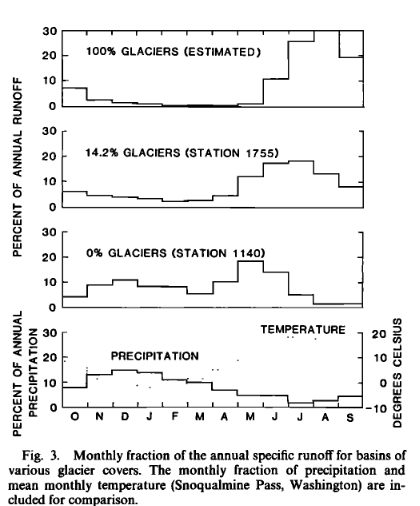
\includegraphics[width=\textwidth]{Plots/fountain_1985_fig3.png}
        \caption{Monthly fraction of the annual runoff for basins of various glacier cover.}
        \label{fig:subfig1}
    \end{subfigure}
    \hfill
    \begin{subfigure}[b]{0.49\textwidth}
        \centering
        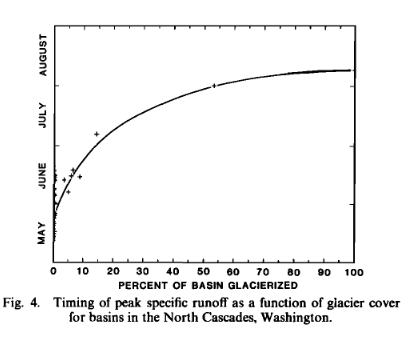
\includegraphics[width=\textwidth]{Plots/fountain_1985_fig4.png}
        \caption{Timing of peak specific runoff as a function of glacier cover.}
        \label{fig:subfig2}
    \end{subfigure}
    \caption{Figures 3 and 4 from Fountain and Tangborn (1985) showing how the percent of basin glacierized delays the peak runoff time of the basin.[Need to change these figs, maybe use fig 2 from that paper]}
    \label{fig:main_figure}
\end{figure}
\FloatBarrier
\subsection{Role of numerical modeling in understanding glacial runoff}
One of the most accurate ways to predict out how glaciers will affect the runoff of a glaciated mountain catchment is by using computer 
models to approximate the water discharge of the glaciers. Scientists have been using computers to model glaciers for several decades, 
such as this paper by Iken A, 1981. As computational resources have grown, these models have grown in complexity and resolution leading 
to very computationally expensive models. These models have proved to be very accurate in modeling the past and present state of a variety 
of glacier types all around the world.

\subsection{Challenges in computational modeling of glaciers}
% AISMs are numerically very sophisticated; these models are also not very intuitive and often take a while to learn how to run. The advantage 
% of AISMs is that they do a particularly good job of modeling ice dynamics. For some glaciers such as marine calving glaciers, accurate ice 
% dynamics are crucial to accurately model them, as shown in Amaral et al., 2020. However, modeling glaciers in 3-dimensions is often 
% unnecessary. If we can use simpler models, such as the Shallow Ice Approximation (SIA) model, to calculate the water runoff of small 
% mountain glaciers in locations such as the Alps, then we can run these models over more glaciers and larger areas, and it is easier to 
% incorporate them into larger hydrology models.
Many of these more advanced models can be quite complex to run due to there being a variety of input parameters and different configurations to run the model. The 
goal of this paper is to write a simple Shallow Ice Approximation (SIA)-Mass Balance model that is easy to run and understand while still 
being reasonably generalizable to different small mountain glaciers. The advantage of using much more advanced models is that they often do 
a much better job at modeling the ice dynamics of glaciers. For some glaciers such as marine calving glaciers, accurate ice dynamics are 
crucial to accurately model them, as shown in Amaral et al., 2020. However on smaller mountain glaciers, modeling in 3-dimensions if often 
unnecessary and simpler models such as the SIA can be used. This paper will compare the results of a simple SIA-Mass Balance model to the 
results of OGGM, a much more advanced model using a simplified version of the Stokes Equations.

\section{Literature Review}
\subsection{Prior research on SIA vs. Stokes models}
    As shown in Le Meur et al., 2004, there are significant differences in computational time between a SIA model and a Stokes model. When 
computing the free surface and associated velocity field, the SIA model took 1 minute of CPU time, whereas the Stokes model took 2 hours. 
This disparity grew even larger for 3D models. The authors show that there are some instances where SIA models do significantly worse than 
Stokes models, such as glaciers on steep slopes and glaciers in steep, narrow valleys because SIA models only approximate the Stokes 
equations. One of these approximations is to ignore horizontal stress gradients. This can cause a SIA model to deviate from a Stokes model 
significantly in predicted glacier flow and expansion. In one example, the resulting SIA model can have an upper free surface that is 
15--20\% greater than the Stokes model and velocities up to a factor of 2 greater (Le Meur et al., 2004). In the 2D model, the bed 
characteristics and slope become the limiting factor of the SIA model; Le Meur et al., 2004 note that the maximum velocity ratio of their 
SIA and Stokes models goes from 1.9 in a 3D model to 1.3 in a 2D model, which will differ depending on model configuration, but it tends to 
indicate that the horizontal stress gradients played a large part in this error. They found instances in which the SIA models performed well 
compared to Stokes models---particularly large flat glaciers with relatively free edges. One thing to note about this comparison study is 
that the authors are looking at the shape, area, and velocity profile of the glacier, whereas this study will focus on the water output 
(surface mass loss) of the glacier.
\subsection{Using SIA models to model alpine glaciers}
    There are several papers, such as Le Meur et al., 2003 and Kessler et al., 2006, that use an SIA model for alpine glaciers. The consensus 
from those papers is that SIA models only work well on alpine glaciers with a low aspect ratio, defined as the thickness-to-extent ratio in 
Le Meur et al., 2004. The glacier used by this study will have a low aspect ratio and therefore a SIA model should work well to model it.
\subsection{Using SIA models to model water runoff from glaciers}
    Additionally, there is precedent for using a SIA-Mass Balance model for modeling water runoff from glaciers (Naz et al., 2014). This paper used 
a SIA model to approximate the ice dynamics and a mass balance model to approximate the accumulation and ablation patterns on the glacier. 
As shown in their paper, the SIA model was able to accurately predict the glacier, and the coupled hydrological model was able to predict 
the stream flow accurately---only overestimating the July flow by an average of 13\% and underestimating the August and September flow by an 
average of 2\%.

\section{Thesis Statement}
How much do ice dynamics affect the model result when modeling small mountain glaciers for water runoff? I theorize that if using a simple 
1-dimensional SIA-Mass Balance model on small mountain glaciers (with a low aspect ratio), the mass balance profile will have a 
much larger effect on the output of the model and its overall accuracy than the modeled ice dynamics. The results of the SIA-Mass Balance 
model and the OGGM model will be compared to the actual stream flow data to verify this hypothesis.
\subsection{Study Site}
\textbf{\large South Cascade Glacier, Washington State}

In this study, I will focus on modeling the South Cascade Glacier in the North Cascades region of Washington State. The South Cascade Glacier is 
roughly 1.68 square kilometers with widths ranging from 400m-1200m, has a mean elevation of roughly 1900 meters, (GLIMS) faces North, an average thickness of 99 meters, and a 
maximum thickness of 195 meters (GlaThiDa Consortium, 2020). The glacier is small, not overly steep (average slope of 7.14 degrees along my 
centerline in 2021), and has a low aspect ratio (thickness to extent ratio), therefore a
SIA model should be able to accurately model its ice dynamics. On the other hand, the glacier is large enough to exhibit some movement 
and produce a measurable amount of runoff throughout the year. 

Thanks to the foresight of the USGS in creating the Benchmark Glacier Program in the 1950s to study and document the South Cascade glacier, 
and eventually four more glaciers, there is an abundant amount of information on these glaciers. Due to this program I was able to 
easily access and use temperature, precipitation, mass balance and DEM data from the USGS. Also as part of this Benchmark Glacier program a 
stream gauge was installed just below the glacier to track the runoff from the basin, the data from which was essential to this project.

\begin{figure}[h!]
    \centering
    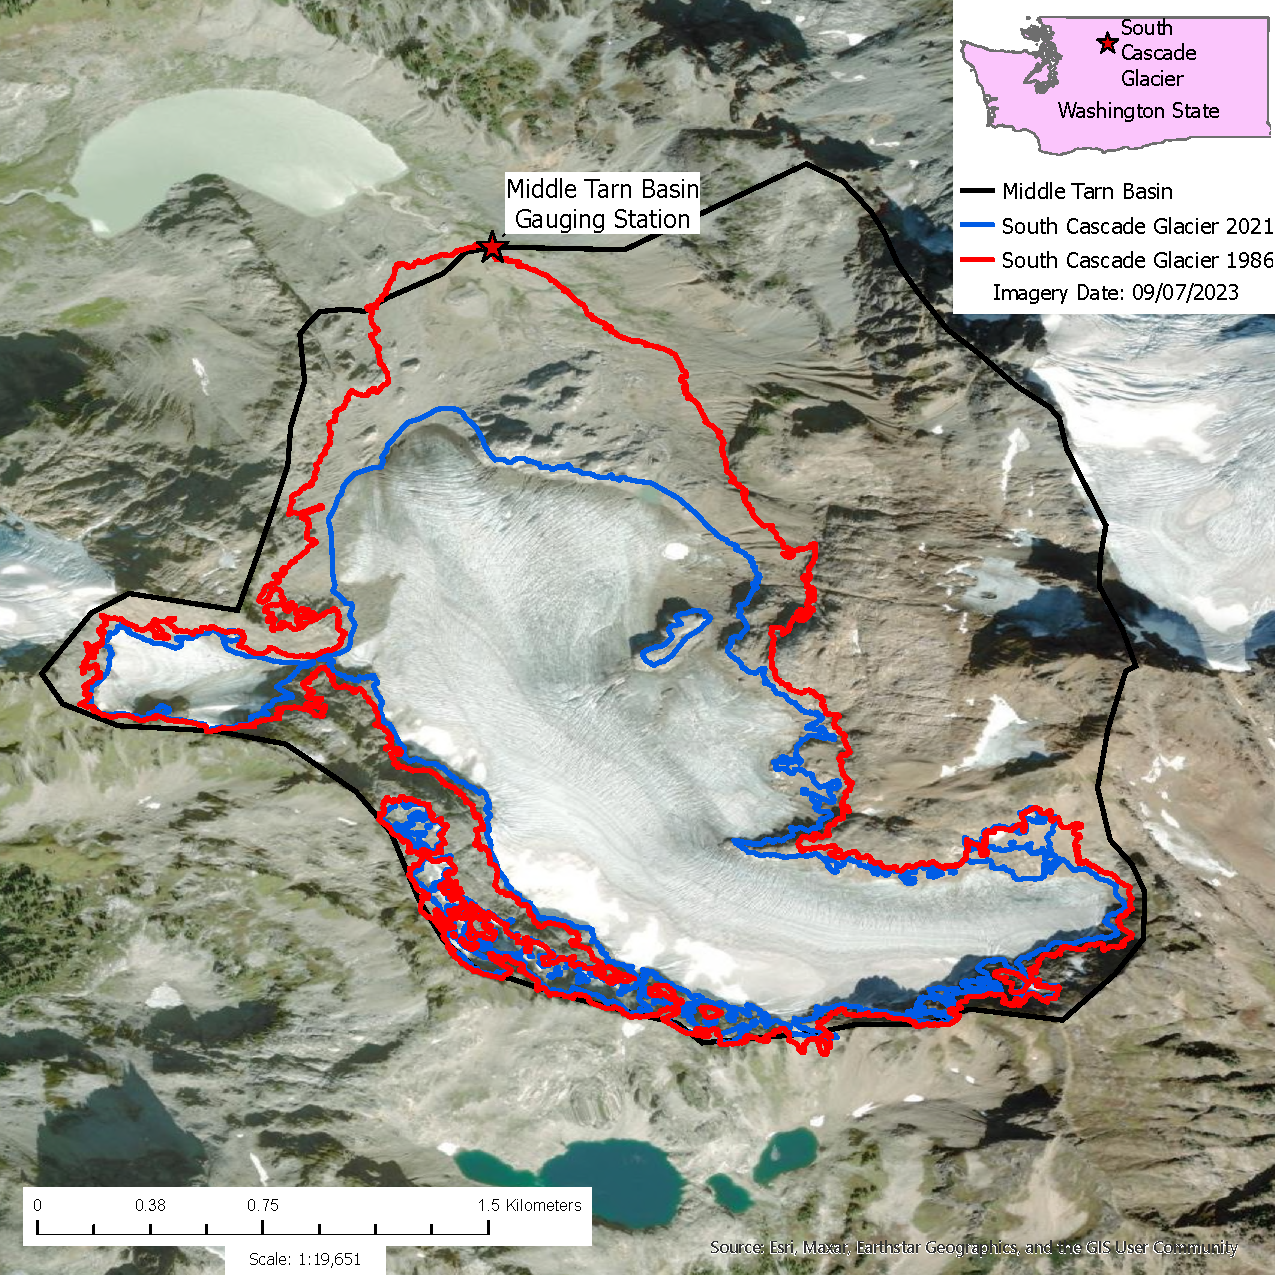
\includegraphics[width=\textwidth]{Plots/SouthCascadeGlacierMap.pdf}
    \caption{Map of the South Cascade Glacier in the North Cascades of Washington.}
    \label{fig:south_cascade_glacier}
\end{figure}
\FloatBarrier

\begin{table}[h!]
    \centering
    \begin{tabularx}{\textwidth}{|c|X|}
        \hline
        Symbol & Description \\
        \hline
        $Z_g$ & Glacier surface altitude (m) \\
        ELA & Equilibrium line altitude (m)\\
        $\gamma$ & Spinup mass balance equation gradient (m/year)\\
        $Y$ & Current year \\
        $Q$ & Ice flux ($\text{m}^2/\text{day}$)\\
        $A$ & Flow rate factor ($5.87*10^{-19}\text{Pa}^{-3}\text{day}^{-1}$) \\
        $n$ & Flow law exponent (3) \\
        $p_{ice}$ & Density of ice ($917\text{kg/m}^3$) \\
        $g$ & Acceleration due to gravity ($9.81\text{ m/s}^2$) \\
        $\frac{\partial z_s}{\partial x}$ & Slope of glacier \\
        $H$ & Ice thickness (m)\\
        $T$ & Temperature ($^\circ$C) \\
        $M_{snow}$ & Snow melt factor ($\text{m water equivalent}/^\circ\text{C}/\text{day}$) \\
        $M_{ice}$ & Ice melt factor ($\text{m water equivalent}/^\circ\text{C}/\text{day}$) \\
        $P$ & Precipitation (m) \\
        $\alpha$ & Precipitation conversion factor \\
        $b_s$ & Summer mass balance (m/day) \\
        $b_w$ & Winter mass balance (m/day) \\
        ${Accum}_{lower}$ & Accumulation lower bound ($\text{m}_{\text{ice}}/\text{m}_{\text{snow}}$) \\
        ${Accum}_{upper}$ & Accumulation upper bound ($\text{m}_{\text{ice}}/\text{m}_{\text{snow}}$) \\
        $S_{depth}$ & Snow depth (m water equivalent) \\
        $S_{melt-vol}$ & Snow melt volume ($\text{m}^3$ water equivalent) \\
        ${Area}_{basin}$ & Basin area ($\text{m}^2$) \\
        ${Area}_{glacier} $ & Glacier area ($\text{m}^2$) \\
        $R_{vol}$ & Rain volume ($\text{m}^3$ water equivalent) \\
        $G_{melt-vol}$ & Glacial melt volume ($\text{m}^3$ water equivalent) \\
        \hline
    \end{tabularx}
    \caption{Symbols Table}
    \label{tab:symbols_table}
\end{table}
\FloatBarrier

\section{Methods}

\subsection{Model Development}
\subsubsection{Model Overview}

% The model is a one-dimensional SIA model coupled with a temperature degree day mass balance model and snow model. 
% The structure of the model is
\textbf{Model Structure:}
\begin{enumerate}[leftmargin=2cm]
    \item Ice dynamics modeled using SIA
    \item Temperature degree day and precipitation mass balance model
    \item Temperature degree day and precipitation (snow fall/melt and rain) model
\end{enumerate}

There are two sections to getting a complete model run, the spinup and the data driven run. The spinup section of the model runs for 500 years and aims to replicate the 
state of the glacier in 1984 when weather data becomes readily available. The spinup run starts with the bed topography and no ice and uses a simple mass balance 
equation to accumulate ice to simulate the glacier state in 1984. The data driven run starts in 1984 with the simulated spinup glacier and applies a temperature and 
precipitation driven mass balance model to model how the glacier changes until 2024. The data driven run also contains the precipitation model to calculate the runoff 
from snow melt and rainfall.

\subsubsection{Spinup run}
This section uses the simple mass balance equation below
\begin{equation}(Z_g-\text{ELA})*\gamma /365.25\end{equation}
This uses a $\gamma$ of 0.0309 to calculate the mass balance in meters per day. When the spinup hits the year 1900 the ELA is shifted up from 1903m to 1930m to simulate the 
retreat state of the glacier. The figure below shows the model in 1958 (474 years of spinup), and 1986 (500 years of spinup and 2 years of data driven run) compared with the actual 
glacier in 1958 and in 1986 derived from a DEM \cite{ref3}. The gaps in the actual glacier lines are due to the available DEMs being partially incomplete over the glacier area.

% Three factors were tuned to create the spinup glacier, the initial ELA, the shifted ELA in 1900 and $\gamma$. These variables were tuned to 
% minimize the average mean squared error (MSE) of the modeled glacier and the actual glacier in 1958 and 1986 when DEM's are available. The result is 
% a MSE of 1.26\% in 1958 and a MSE of 0.99\% in 1986.

% The data driven run uses the mass balance model described below to calculate the mass balance for the glacier instead of the simple mass balance 
% equation used for spinup. This mass balance model is driven by temperature and precipitation data. The data driven run also contains a precipitation 
% model in order to calculate the snow fall and melt and rainfall in the basin.

\subsubsection{Data driven run setup}
The data driven section of the model run relies on a variety of data in order to run. It requires daily temperature and precipitation data, 
a bed topography, yearly glacier area, and total basin area to run. In order to tune the input parameters the model needs winter and summer mass balance 
data. The model needs seven input parameters to run: ice melt factor, snow melt factor, temperature lapse rate, start accumulation factor, end 
accumulation factor, avalanche percentage and precipitation conversion factor. 

The centerline bed topography was calculated using latitude, longitude and elevation bed topography from Robert Jacobel \cite{ref4}. 
% This  was calculated using ground penetrating radar.
 I used the ArcGIS Kriging Interpolation function \cite{ref5} to interpolate this point elevation data into a complete 
bed topography across the whole glacier. I then traced a line down the center of the glacier using the interpolated bed and got bed elevation points for the line 
from the interpolated data. I then used these new latitude, longitude, and elevation points to create the one-dimensional bed topography for 
the model. I explored using a centerline from RGI 7.0 \cite{ref6}, but ultimately chose not to use it because the RGI centerline did not go 
down the center of the interpolated bed.

\subsubsection{Ice Dynamics}
\paragraph{SIA Model}

The SIA model is a one-dimensional model that uses the shallow ice approximation to approximate the ice dynamics of the glacier. This model 
calculates the one dimensional ice flux of the glacier using equation 2. 
\begin{equation}Q=\frac{2A}{n+2}(p_{ice}g|\frac{\partial z_s}{\partial x}|)^n\frac{H^5}{5}\end{equation}
% This model works by creating an array of bins that represent the glacier. The model then calculates the ice flux of each bin and uses that to 
% create the flow of ice in the model. 
\paragraph{Assumptions}

The SIA ice flux equation make several assumptions. First, the equations are 1-dimensional, so they neglect longitudinal stress, and ice only 
flows downhill. Second, the equations also assume that there is no basal sliding of the glacier. Third, the equations only use gravity as the 
driver of ice flow; they ignore other forces such as lateral and basal stress. Fourth, this set of equations assumes that the horizontal 
dimensions of the modeled glacier are much larger than the vertical dimensions.

\subsubsection{Mass Balance Model}
The mass balance of the glacier is calculated using temperature and precipitation data from the Diablo Dam weather station at 272m. The 
temperature at the glacier is calculated by using a month-specific lapse rate. 
% This month-specific lapse rate was empirically calculated using data from the Diablo Dam weather station and the South Cascade Glacier weather station at 1830m from 2010-2018. 
The precipitation at the glacier is calculated by multiplying the precipitation at the Diablo Dam weather station by the precipitation conversion factor of 1.58 
obtained from (reference). The ablation of the glacier is calculated by using a combination of an ice melt factor and a snow melt factor. Above the ELA the 
ablation is calculated by equation 3 for $T>0$
\begin{equation}b_s=T*M_{snow}\end{equation}
Below the ELA the ablation is calculated by equation 4 for $T>0$
\begin{equation}b_s=T*(M_{snow}+((ELA-Z_g)/(ELA-min(Z_g)))*(M_{ice}-M_{snow}))\end{equation}
The result of this equation is the snow melt factor being used at the ELA and a linear increase in the melt factor until it hits the ice melt 
factor at the base of the glacier. This set of equations assumes that in the accumulation zone (above the ELA) the surface is always snow year 
round, and below the ELA the surface transitions from snow to ice as you decrease in elevation.
The accumulation of the glacier is calculated using equation 5 for $T<0$
\begin{equation}b_w=P*\alpha*({Accum}_{lower}+((Y-1984)/(2024-1984))*({Accum}_{lower}-{Accum}_{upper}))\end{equation}
This equation starts the accumulation factor at $Accum_{lower}$ at the start of the data driven run in 1984 and linearly increases it to $Accum_{upper}$ by the end 
of the run in 2024.

\subsubsection{Precipitation Model}
\paragraph{Snow Model}
The snow melt model uses precipitation and temperature data to accumulate and melt snow. 
% This model uses 14 elevation bins and keeps track of the snow depth in each bin. Each elevation bin has a corresponding area that represents the area of the basin in the bin's elevation range. 
The equation below is used to calculate the change in snow depth per timestep 
\begin{equation}S_{depth} += 
\begin{cases} 
  P*\alpha & T \leq 0,\\
  -\text{min}(|M_{snow}*T|,S_{depth}) &  T > 0
\end{cases}\end{equation}
The snow melt is constrained so that there cannot a negative snow depth. 
The total volume of snow melt is calculated by equation 7.
\begin{equation}S_{melt-vol}=(M_{snow}*T)*({Area}_{basin}-{Area}_{glacier})\end{equation}
This give us the total volume of snow melt on the non-glacierized areas of the basin. Any snow that falls on the glacier is factored into 
the glacier mass balance equations and accumulated on the glacier.
\paragraph{Rain Model}
The rain is simply modeled by $P*\alpha$ for positive temperature days. The volume of rain is calculated equation 8
\begin{equation}R_{vol}=P*\alpha*{Area}_{basin}\end{equation}
This calculates the rain for the whole basin because rain is not factored into the glacier mass balance. This assumes that  that any rain 
that falls runs out of the basin on the day it falls.

\paragraph{Avalanche Model}
In order to stop snow accumulating to unrealistic depths at high elevations an avalanche model is used. This model avalanches the 
snow above 2123m once per year on a randomly chosen date (chosen each year) between January and March. The amount of snow that 
avalanches is controlled by the avalanche percentage. On the chosen that the snow depth above 2123m is decreased by the avalanche 
percentage and that snow is evenly distributed below 1900m. The result of this is the average snow depth approximately 2m water 
equivalent in September and October before starting to accumulate again. With an avalanche percentage of 0 it is approximately 5.5m water 
equivalent in September and October. This decrease in snow depth leads to a more realistic model and improves the accuracy of the runoff 
model by roughly 1 percentage point. This is caused by there being more snow available for melt at the lower elevations where the 
temperature is higher.

\subsubsection{Glacial Melt Model}
The glacial melt model uses the mass balance of the glacier to calculate how much volume the glacier is losing. The volume of runoff from the 
glacier is calculated by the equation
\begin{equation}G_{melt-vol}=b_s*{Area}_{glacier}\end{equation}
\subsection{Model Calibration}
\subsubsection{Data used for model}
The temperature and precipitation data used for the model is from the Diablo Dam weather station at 272m. The data is available from 1984-2024 
and missing 298 days of temperature measurements and 292 days of precipitation measurements. The missing temperature data was interpolated 
using the interp function from the numpy python library \cite{ref7}, the missing precipitation data was assumed to be 0. The glacier area data used in 
the model is from the USGS \cite{ref8}. The basin area data was calculated using a DEM from the USGS and the basin outline shown in figure 1.
\textbf{talk about how the lapse rate is calculated}
\subsubsection{Calibration}
% The spinup initial ela, ela shift and gamma were manually optimized to match the glacier extent in 1984. 
\paragraph{Spinup Calibration}
The spinup initial ELA, ELA in 1900 and $\gamma$ were optimized using the minimize function with the Nelder-Mead method from the scipy library \cite{ref9}.
The optimization was done by minimizing the relative RMSE (equation 10) of the glacier's in 1958 and 1986. The sum of the cross-sectional area of the glacier was used to calculate the RMSE. This metric was chosen to create a glacier with an cross-sectional area as close to the actual glacier as possible. 
The result is a relative RMSE of 6.95\% with RMSE's of 7.27\% and 6.63\% in 1958 and 1986 respectively.

\begin{equation}
    \mathrm{RMSE} = \left(\frac{\sqrt{\left( O^{1958}_i - S^{1958}_i \right)^2}}{{O^{1958}}}+\frac{\sqrt{ \left( O^{1986}_i - S^{1986}_i \right)^2}}{{O^{1986}}} \right)/2*100
\end{equation}

\noindent where:
$$O = \text{Measured sum of cross-sectional area}, \quad S=\text{Modeled sum of cross-sectional area}$$

\begin{figure}[h]
    \centering
    \begin{subfigure}[b]{0.49\textwidth}
        \centering
        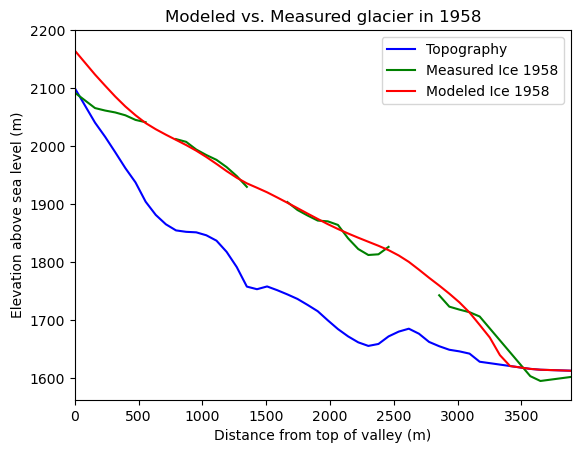
\includegraphics[width=\textwidth]{Plots/1958_glacier_comparison.png}
        \label{fig:1958_glacier_comparison}
    \end{subfigure}
    \hfill
    \begin{subfigure}[b]{0.49\textwidth}
        \centering
        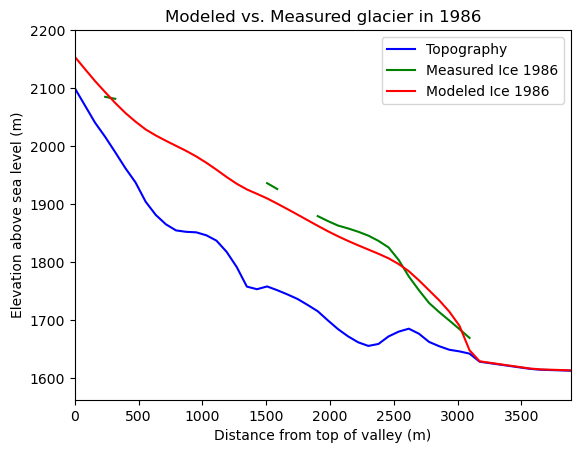
\includegraphics[width=\textwidth]{Plots/1986_glacier_comparison.png}
        \label{fig:v}
    \end{subfigure}
    \caption{Glacier from DEM compared with modeled glacier in 1958 and 1986}
    \label{fig:1986_glacier_comparison}
\end{figure}
\FloatBarrier

Looking at these figures the difference in the actual glacier vs the modeled glacier at the top of the valley stands out. The modeled glacier is much thicker in this 
location compared to the actual glacier. This may be due to different accumulation patterns on the actual glacier compared to the model. 
\textbf{Note that this could also be due to error in bed topo}

\paragraph{Summer Mass Balance Calibration}
The two input parameters that control the summer mass balance are the ice melt factor and the snow melt factor. They were calibrated using yearly summer 
mass balance data available from the USGS from 1984-2024. I used the minimize function 
to minimize the mean squared error between the modeled mass balance and the USGS measured mass balance. 
\paragraph{Winter Mass Balance Calibration}
There are also two factors that control the winter mass balance, the start and end accumulation factors. They were tuned using the same 
method as the summer mass balance factors using the USGS yearly winter mass balance data available from 1984-2024.
\textbf{Maybe add some thoughts on why the amplitudes are off}
\textbf{Put the two graphs on the same scale}
\begin{figure}[h]
    \centering
    \begin{subfigure}[b]{0.49\textwidth}
        \centering
        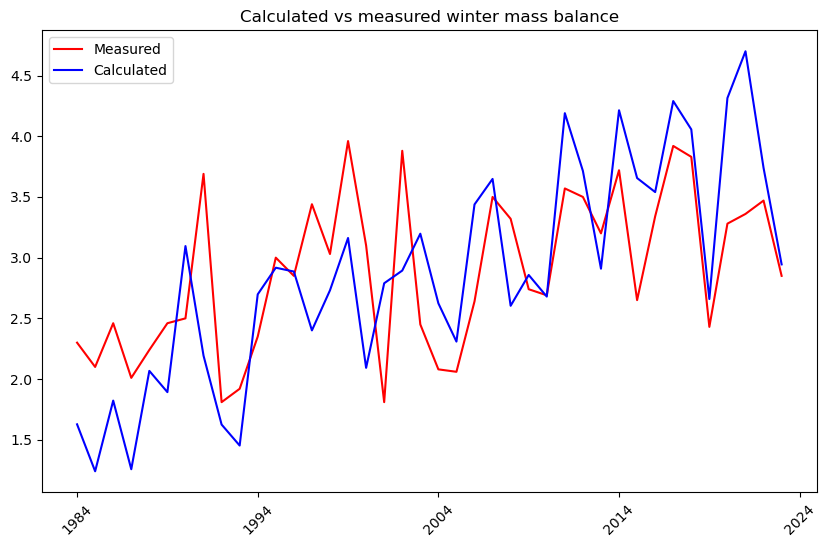
\includegraphics[width=\textwidth]{Plots/winter_mb_compare.png}
        % \caption{Spinup comparison of the model in 1986 after 500 years of spinup and 2 years of run compared with the actual glacier in 1986.}
        \label{fig:winter_mb_compare}
    \end{subfigure}
    \hfill
    \begin{subfigure}[b]{0.49\textwidth}
        \centering
        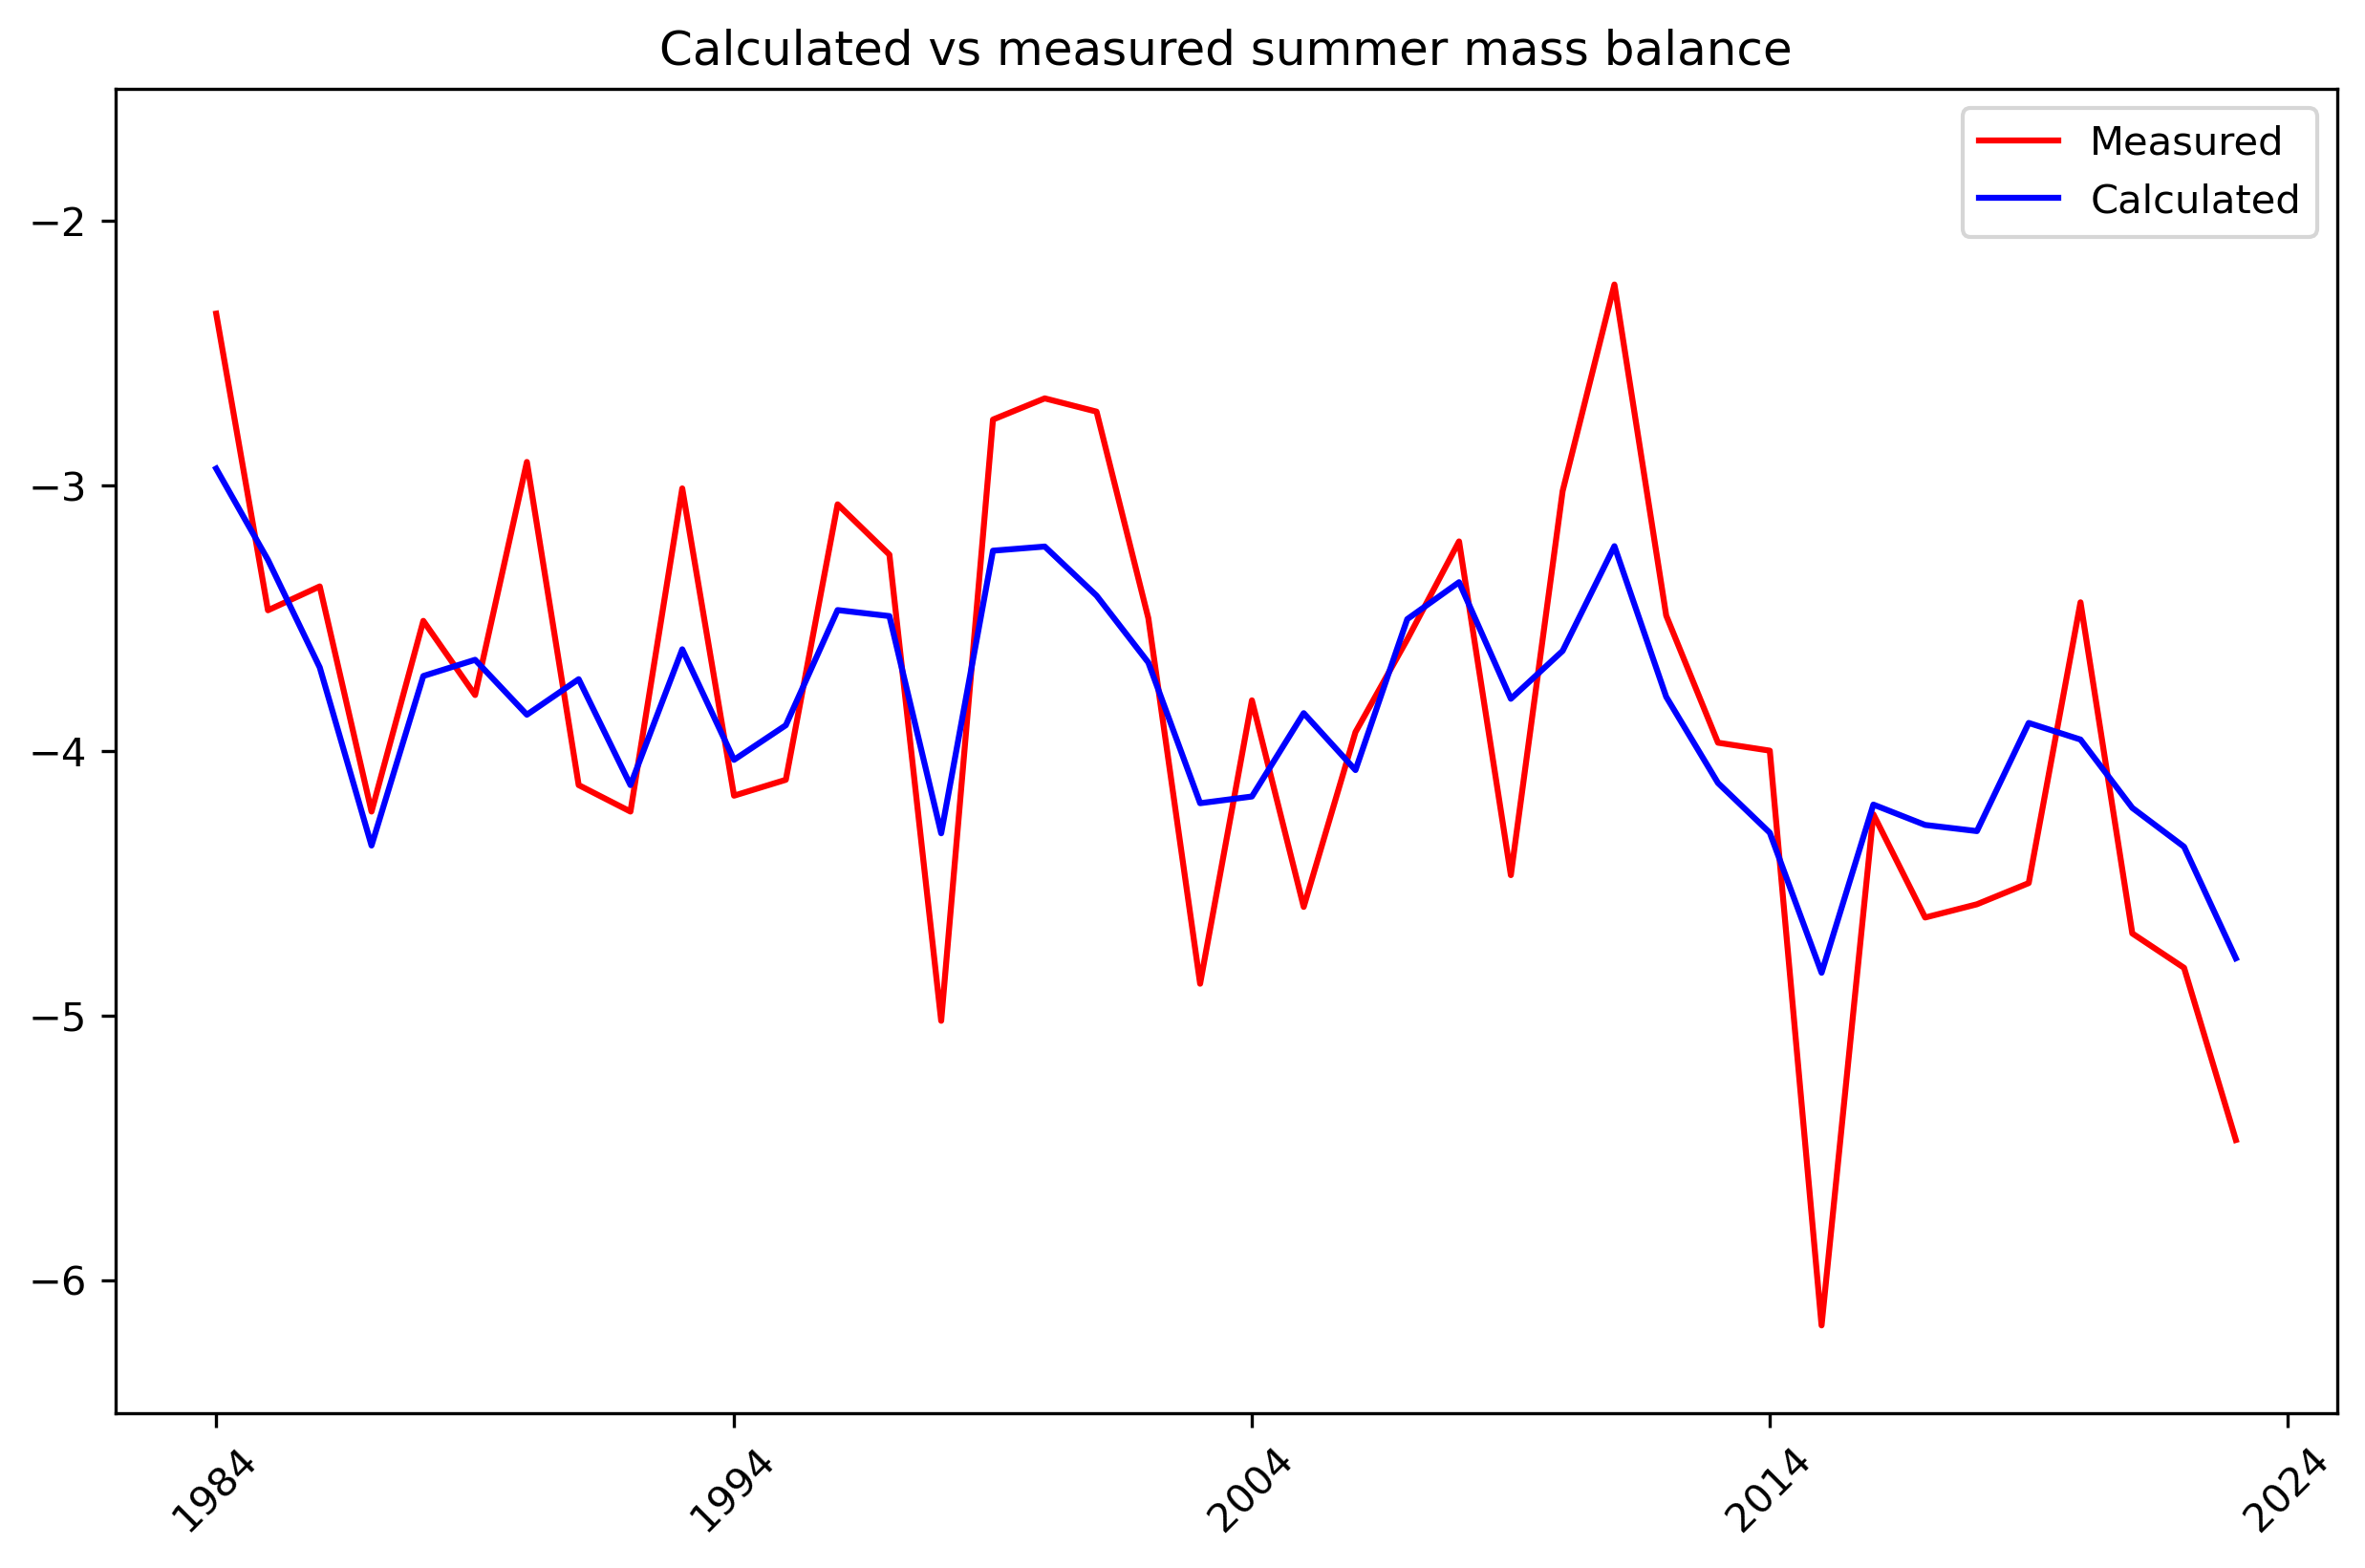
\includegraphics[width=\textwidth]{Plots/summer_mb_compare.png}
        % \caption{Timing of peak specific runoff as a function of glacier cover.}
        \label{fig:summer_mb_compare}
    \end{subfigure}
    \caption{Comparison plots of the calculated vs measured winter and summer mass balance.}
    \label{fig:mb_comparison}
\end{figure}
\FloatBarrier

\paragraph{Avalance Percentage Calibration}
The avalanche percentage was optimized using the same minimize function as the mass balance parameters. Instead of minimizing the MSE, the mean of the 
snow depth over the whole data driven run (1984-2024) was minimized. The mean snow depth was minimized because the almost all of the snow on the 
non-glacierized areas of the basin should melt during the summer. By minimizing the mean snow depth over the whole run, the snow depth during 
the summer will be minimized since the avalanche percent cannot change the amount of snow present in the whole basin, just the elevation it is at. If 
there is more snow at lower elevations then more snow will melt during the summer.
\textbf{explain better}
% The figure below shows the resulting ice thicknesses computed by the model in 2021 compared to the 2021 DEM.
% \begin{figure}[h!]
%     \centering
%     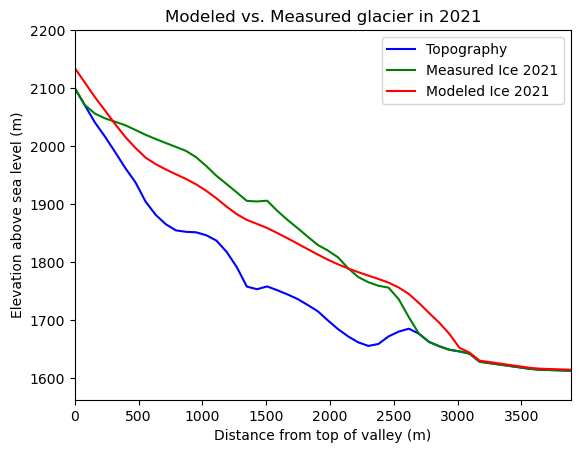
\includegraphics[width=\textwidth]{Plots/2021_glacier_comparison.png}
%     \caption{Model comparison of the ice thickness in 2021 compared to the actual glacier in 2021.}
%     \label{fig:2021_glacier_comparison}
% \end{figure}
% \FloatBarrier
% \begin{figure}[h!]
%     \centering
%     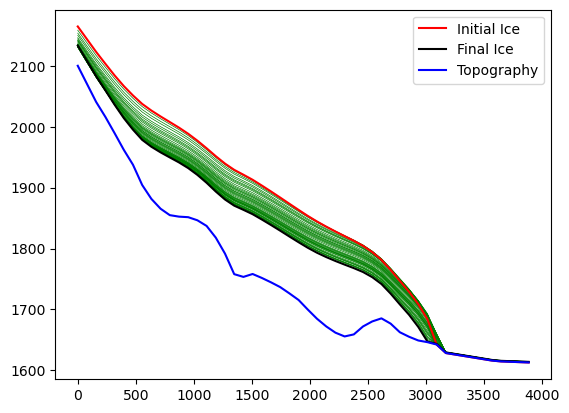
\includegraphics[width=\textwidth]{Plots/model_run_1984_2024.png}
%     \caption{Output of the model run from 1984-2024.}
%     \label{fig:model_run_1984_2024}
% \end{figure}
% \FloatBarrier
\subsubsection{Model Comparison}
\paragraph{Running OGGM Model for the South Cascade Glacier}
The OGGM model was run using the run\_with\_hydro task from the oggm library. This model run used the GSWP3\_W5E5 historical temperature and 
precipitation data \cite{ref10} to model the hydrology of the glacier from 1984-2019. The total runoff from the glacier was calculated using 
runoff from the glacier using the melt\_on\_glacier\_monthly, and liq\_precip\_on\_glacier\_monthly variables. In order 
to calculate the runoff from the non-glacierized areas melt\_off\_glacier\_monthly, and liq\_precip\_off\_glacier\_monthly variables were averaged over the 
SIA model glacier basin area. 

\section{Results}
\subsection{Accuracy of SIA Model}
The calculated runoff of the SIA-Mass Balance model was validated using measured streamflow data from 1992-2007, consisting of 2418 
data points, which were aggregated into 91 months (reference list of papers). This data was measured using 
a stream gauge located just below the glacier (refer to Figure 1 for location). The data is in units of mm per day averaged over the basin area (4.46$\text{km}^2$). This was  
converted to cubic meters per day and then 
summed over the month to calculate a monthly runoff. Not every month was complete, so in order to validate the model, the model runoff was saved 
for the same days as the measured data and then a daily average was calculated for each month. 
This paper will look at the model error in terms of daily average runoff per month due to the several incomplete months of data. 
This paper will used 
three types of error to evaluate the model, relative Root Mean Square Error (RMSE), Nash–Sutcliffe Efficiency (NSE), and Kling–Gupta Efficiency 
(KGE), defined by the equations below. 
\begin{equation}
    \mathrm{RMSE} = \frac{\sqrt{\frac{1}{N}\sum_{i=1}^{N} \left( O_i - S_i \right)^2}}{\bar{O}}*100,
\end{equation}

\begin{equation}
    \mathrm{NSE} = 1 - \frac{\sum_{i=1}^{N}\left( O_i - S_i \right)^2}{\sum_{i=1}^{N}\left( O_i - \bar{O} \right)^2},
\end{equation}

\begin{equation}
    \mathrm{KGE} = 1 - \sqrt{ (r-1)^2 + (\alpha-1)^2 + (\beta-1)^2 },
\end{equation}

\noindent where:
$$O = \text{Observed data}, \quad S=\text{Simulated Data}$$
$$r = \mbox{Correlation coefficient}, \quad \alpha = \frac{\sigma_S}{\sigma_O}, \quad \beta = \frac{\mu_S}{\mu_O}$$
The results for these three methods are 29.26\%, 0.81 and 0.88 respectively. It is important to note that this error is primarily the model error for 
May-November due to the lack of runoff data outside of those months. There is one instance of January, February, March and April, and six 
instances of December. What is interesting about this model is how good it does on longer 
timescales. The relative RMSE of the daily average runoff per year drops to 15.21\%, and the average relative error
for the whole time period is 4.51\%, which shows that over longer time periods the over and underestimates of the model cancel each 
other out and the model becomes more accurate. [Compare to Naz paper, note that the precip model they use is more complicated]
\begin{figure}[h!]
    \centering
    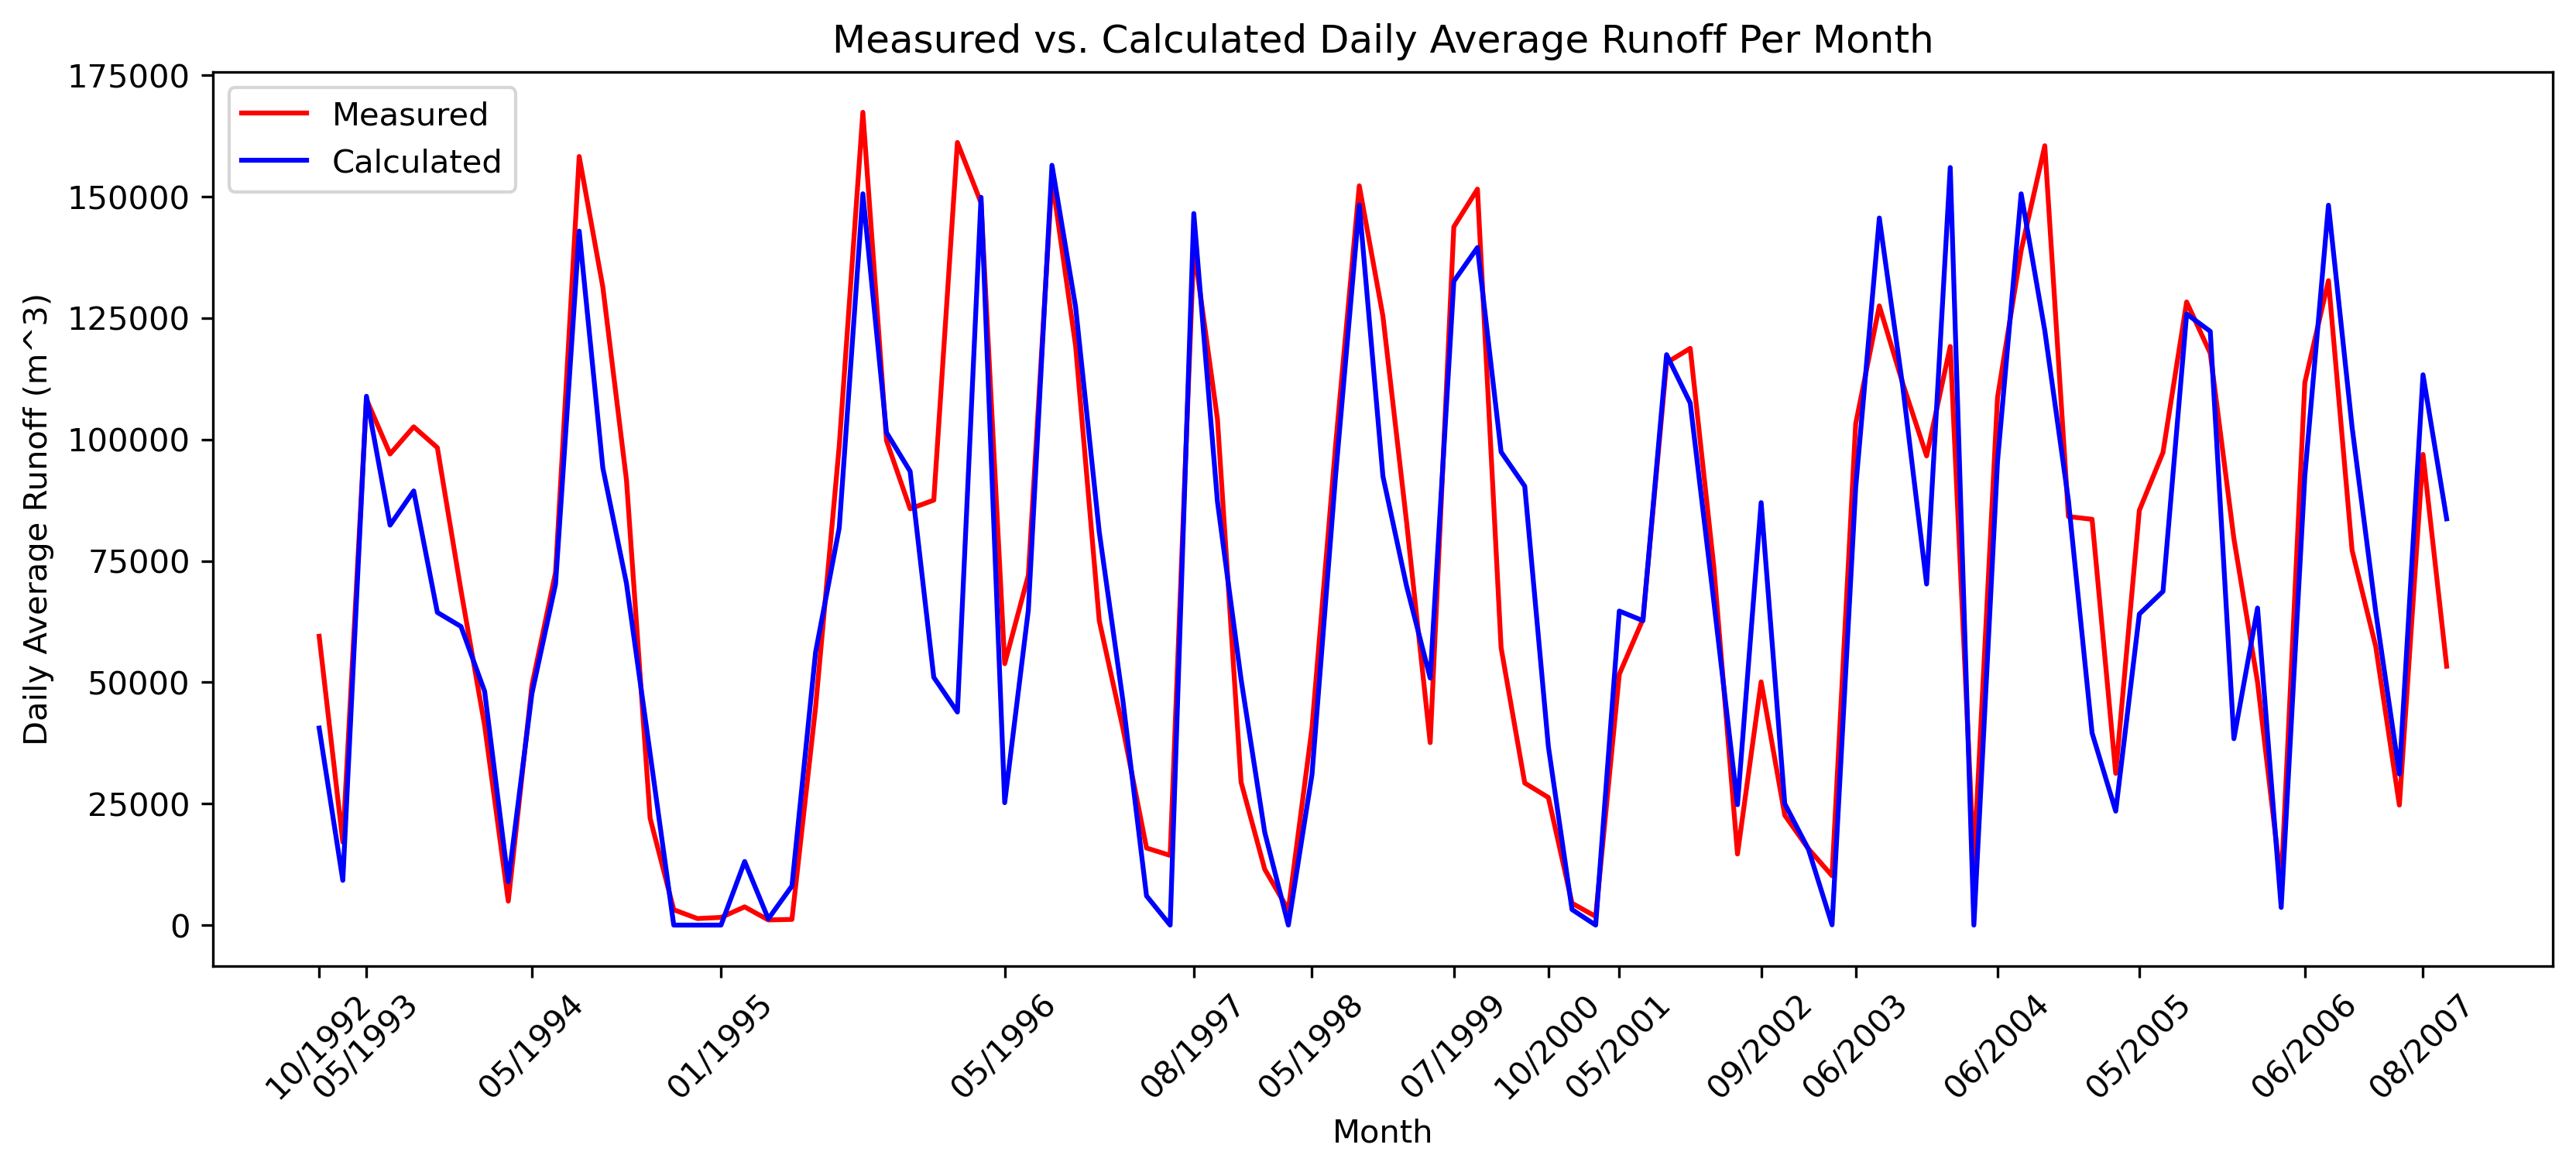
\includegraphics[width=\textwidth]{Plots/calc_vs_measured.png}
    \caption{Measured vs. Calculated runoff data from 1992-2007}
    \label{fig:calc_vs_measured}
\end{figure}
\FloatBarrier
\subsection{Accuracy of OGGM}
The RMSE, NSE and KGE of the OGGM model are 45.96\%, 0.53 and 0.72 respectively. The OGGM Model proved to be slightly less accurate when 
compared to the real-world measured runoff data. OGGM uses the GSWP3\_W5E5 climate modeled data instead of measured temperature and precipitation 
data due to the purpose of the model being to model glaciers into the future.
\begin{figure}[h!]
    \centering
    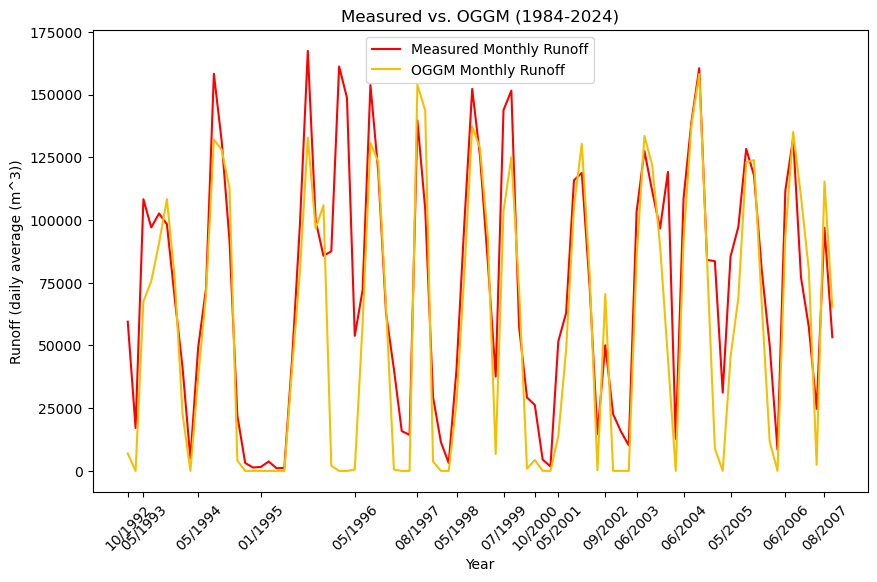
\includegraphics[width=\textwidth]{Plots/oggm_vs_measured.png}
    \caption{Measured vs. Calculated runoff data from 1992-2007}
    \label{fig:oggm_vs_measured}
\end{figure}
\FloatBarrier
\subsection{Comparison of Accuracy}
% The accuracy of the simpler SIA-Mass Balance model is quite impressive compared to the much more advanced OGGM model. The SIA-Mass Balance 
% model's accuracy is roughly two times better than OGGM which is quite impressive. The OGGM model was run on modeled climate data instead of 
% real-world measured data which most likely contributed to its worse accuracy. 
The SIA-Mass Balance model is roughly 1.4 times (averaged over the three error metrics) more accurate than the OGGM model. One reason for the 
higher accuracy of the SIA-Mass Balance model is likely due to it 
using real-world temperature and precipitation data and OGGM using modeled climate data which is less accurate. The SIA model input 
parameters are also tuned to the local climate of the glacier.

\begin{figure}[h!]
    % \centering
    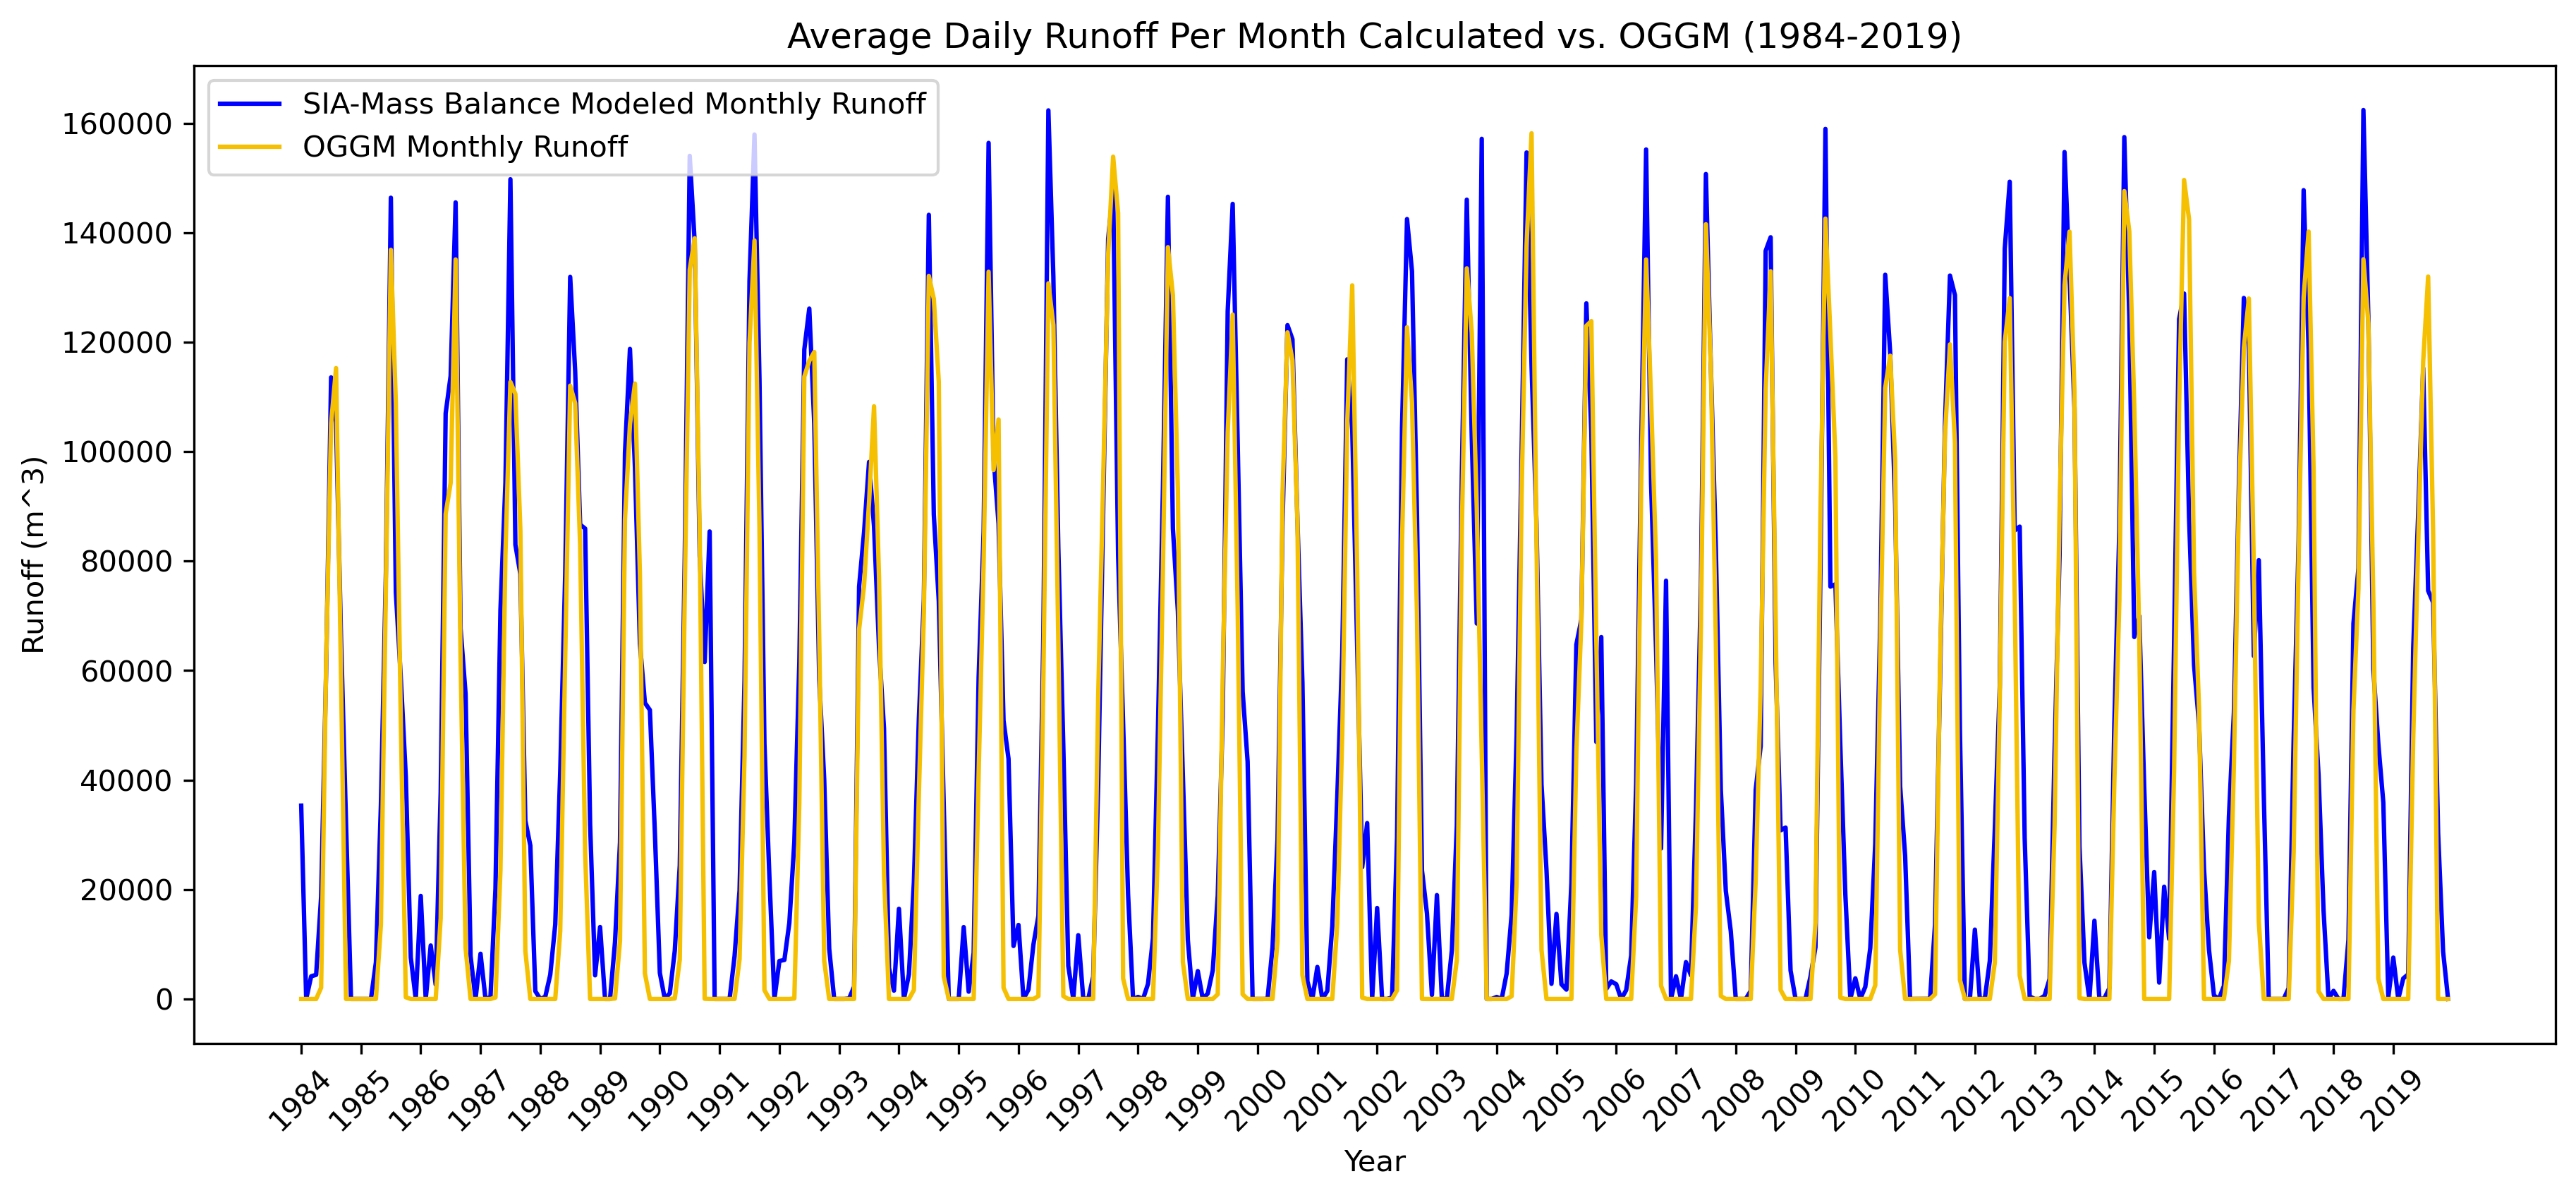
\includegraphics[width=1.3\textwidth]{Plots/oggm_vs_calculated.png}
    \caption{OGGM calculated daily average runoff per month compared to SIA-Mass Balance Model from 1984-2019}
    \label{fig:oggm_model_run_1984_2019}
\end{figure}
\FloatBarrier

\section{Implications of Research}
\subsection{Importance of Simplified Ice Dynamics in Numerical Glacier Modeling}
These results show that complicated and computationally intensive mass balance and ice dynamics are not required to accurately model the 
runoff from small mountain glaciers. This means that we can use much simpler and less computationally intensive models such as the ones used 
in this paper to model the runoff from mountain glaciers much quicker than more complicated models. The modeling techniques used in this paper could 
easily be scaled to a much larger region if mass balance is available to tune the input parameters. Also the relative simplicity of the model used in 
this paper means that it is much easier to modify to add new features and customize to a specific region or glacier.
\paragraph{}
This point is further proved by the error of the SIA-Mass Balance model not changing significantly (less than 0.01 for the KGE and NSE, and less than 
0.1\% for the relative RMSE) when 
the ice flux is set to 0. This means that the ice dynamics of the glacier are not a significant factor contributing to the glacier runoff. One reason 
for this is the South Cascade Glacier is in an active state of retreat which can be seen in the model and the 
glacier outline in Figure 1. Since it is retreating, the model does not need the ice dynamics in order to move more glacier ice into the ablation zone 
where it can melt, much of the glacier is already in this ablation zone.
% I would hypothesize that the input parameters used 
% in my model of the South Cascade Glacier could be used for a much larger model over a similar region as almost all of the input parameters are 
% climate dependent, but this is a topic for another paper. 
\subsection{Applications}
The work of this paper shows that complex ice dynamics and precipitation models are not always required to accurately model the runoff from small mountain glaciers. This 
can have applications in everything from regional glacier modeling to water resource management as glaciers are a significant source of water 
for many communities around the world. 

% \section{Discussion Notes from talking with Dad}
% \begin{enumerate}
%     \item MSE is not a good way to look at error
%     \item Look at the kinds of errors other papers use for similar runoff models
%     \item Look at daily averages per month to reduce variation
%     \item Use relative RMSE to look at error, use np.sqrt(np.sum(error)**2) for RMSE
%     \item Don't reference 2 standard deviations, use 1
%     \item Qualify what I mean by the $R^2$ being good, good compared to what
%     \item Look into what KGE means more
%     \item MAE is actually just error
%     \item Error is basically just for may-october because that is when I have data
%     \item Look at error per days in the month
%     \item Large error in 11/1995 in runoff data is most likely due to the actual precip falling as rain but my model predicting it as snow due to 
%     low temps
%     \item Is error higher when temps are +/- 5 degrees of 0 [No, there is no correlation]
%     \item Note average error for runoff, but a lot of variation
% \end{enumerate}

\section{Discussion}

\subsection{Improvements}
\textbf{mention lapse rate error and how that can effect precipitation error}
The largest problem with the runoff model lies with the precipitation model. This model calculates the type of precipitation that falls (rain or 
snow), based on the temperature. It assumes that if the temperature is greater than $0^\circ$ Celsius then the precipitation is rain, and if the 
temperature is less then $0^\circ$ Celsius then then precipitation is snow. This is a good generalization, but it isn't always true. Looking at the 
error graph, there is a large spike in the error in November of 1995. This is likely due to the model predicting the large amount of precipitation 
during that month falling as snow because the temperatures are just below $0^\circ$ Celsius, but in reality it most likely fell as rain. This also 
highlights the types of error that can be caused by using a proxy weather station that is not present at the glacier such as this model used. With 
more accurate temperature data for the glacier, then the model might correctly predict the precipitation falling as rain. 
\paragraph{}
It is also important to note that out of the 298 missing days of temperature and 292 missing days of precipitation 63 days of temperature and 64 
days of precipitation were during the 1992-2007 period where runoff data is available. Most notable of these missing days is the month of September 
1997. This entire month is missing temperature and precipitation data, and this entire month is included in the measured runoff data. Looking at the 
error for the month it has a relative RMSE of 30.51\% which is very close to the overall relative RMSE of 29.26\%. This 
means that the error this month is quite typical for the model. The interpolated temperatures for this month range from $10^\circ$ C to $5^\circ$ 
during the month, so the glacier is melting and no glacier accumulation is missed. Also from looking at Figure 10, during September glacier melt is 
contributing the majority of the runoff to the basin, so having zero precipitation in the model for September 1997 would not cause as much error as 
if there was no precipitation for December or January when lack of snowfall could affect the runoff in the following summer.
\paragraph{}
These two examples illustrate that missing precipitation data may be much more detrimental to model accuracy than missing temperature data, partly 
due to temperature data being much easier to interpolate than precipitation data.
\subsection{What we can learn from the model results}
Even though the glacier is contributing slightly less than half of the total basin runoff on average (47.56\%), it contributes much more during the summer 
months as show in figure 11. As the glacier retreats it will start contributing less water to the basin runoff resulting in a decrease in total 
basin runoff. If the precipitation stays constant over time, but the glacier continues to retreat the basin runoff will see a steep decline 
particularly in early summer and fall when the glacier contributes most to the runoff. This is especially important considering that the 
Cascades see the least amount of precipitation during that portion of the year as shown in figure 12.
\textbf{the glacier melt percent includes snow melting off the glacier}
\begin{figure}[h]
    \centering
    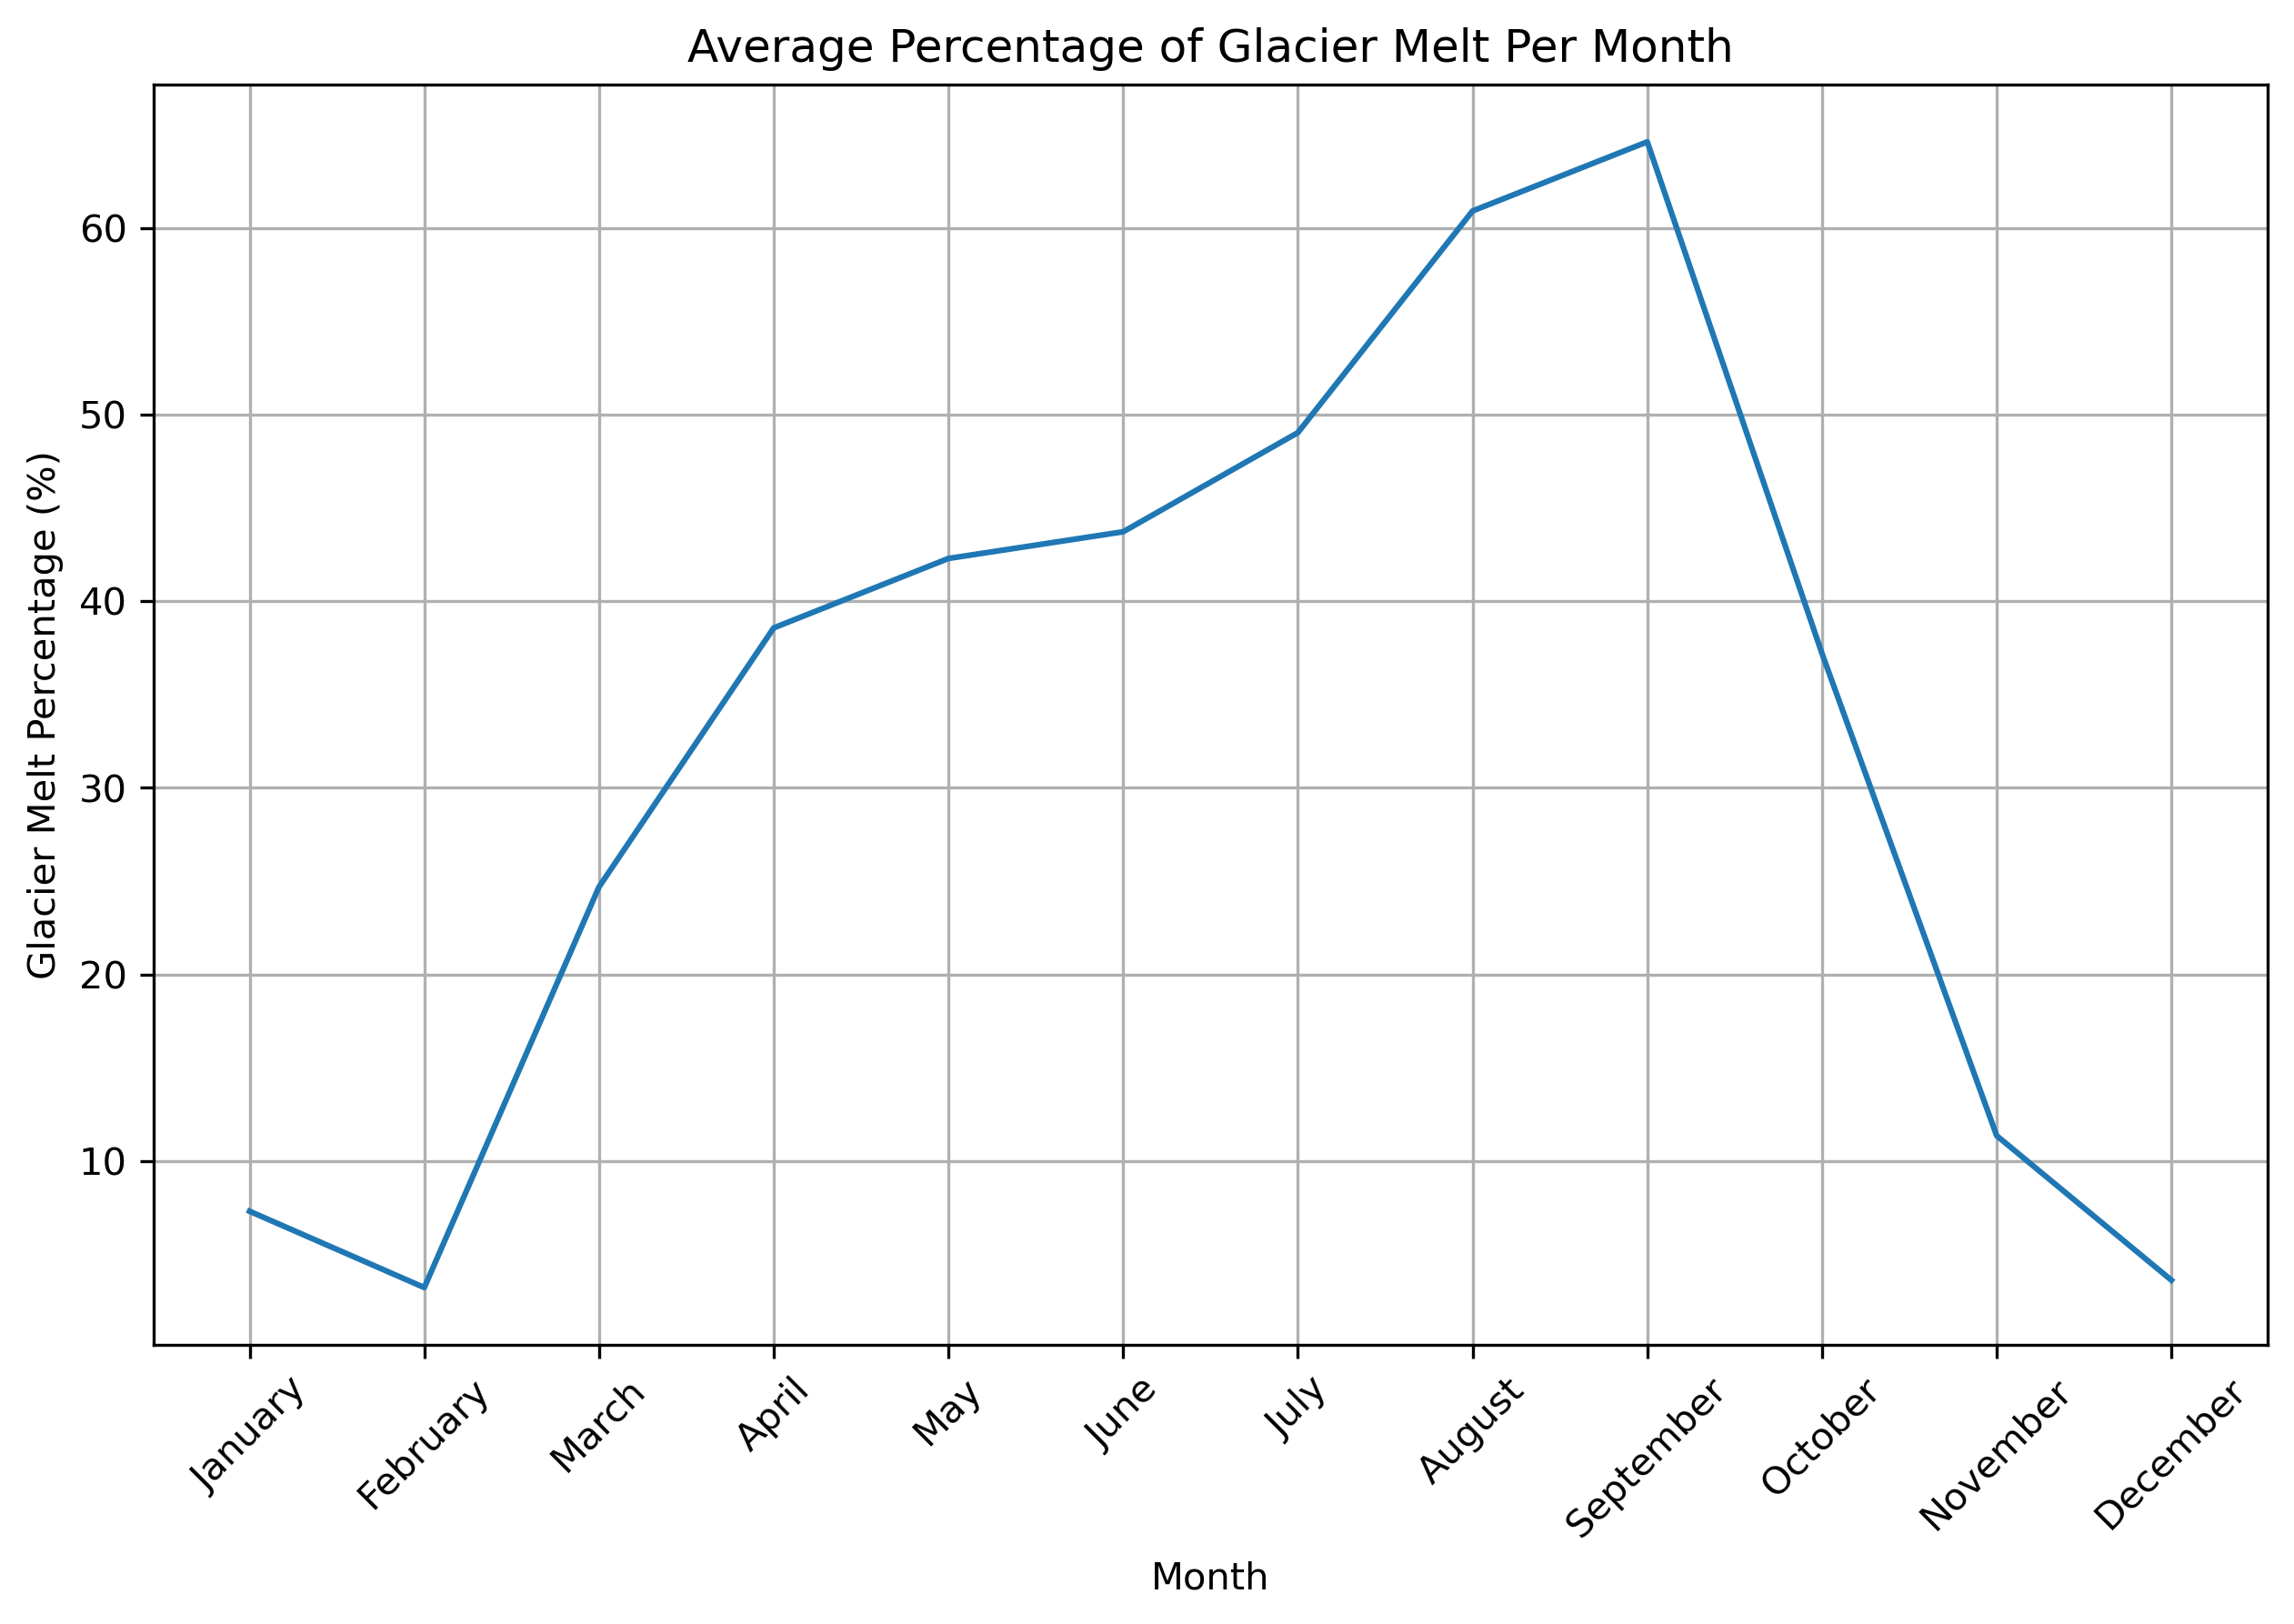
\includegraphics[width=\textwidth]{Plots/percent_glac_melt_month.png}
    \caption{Average percentage from 1984-2024 that the glacier contributes to the monthly runoff}
    \label{fig:percent_glacier_runoff}
\end{figure}
\FloatBarrier\

\begin{figure}[h]
    \centering
    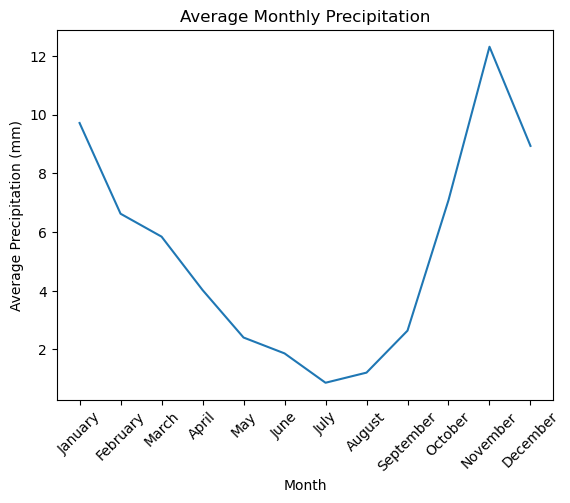
\includegraphics[width=\textwidth]{Plots/monthly_precip.png}
    \caption{Average amount of precipitation per month from 1984-2024 at the Diablo Dam weather station. The average temperature from October-April is below $0^\circ$ C, so the precipitation during those months is mostly snow}
    \label{fig:monthly_precip}
\end{figure}    
\FloatBarrier

\subsection{Mass Balance model error}
The relative RMSE of the winter and summer mass balance are 19.01\% and 13.33\% respectively.
\paragraph{}
Looking at the missing temperature and precipitation one can note a few interesting things about the mass balance model error. There are five years 
with significant gaps (at least one month of missing data) in the temperature and precipitation data. These years are 1984 (missing December), 
1985 (missing January), 1987 (missing July), 1997 (missing March and September) and 2009 (missing May-July). The year with the highest error in 
winter mass balance is 1997 probably due to it missing March data. The measured winter mass balance that year is 3.44m, and the model calculated a 
winter mass balance of 2.65m. One possibility for this is that there was a large amount of snowfall during March of that year, but since the 
precipitation data is missing for that month, the glacier accumulation is 0. According to PRISM (reference) the South Cascade Glacier recieved 0.57m 
of precipitation during March 1997. Using the mass balance equations above, the accumulation on the glacier during March 1997 with 0.57m of 
precipitation would be 1m, which would increase the winter mass balance for that year form 2.65m to 3.65m, much closer to the measured value. This 
illustres just how important consistent and reliable weather data is for models like these because a month of missing weather data can skew the 
result. 
% \subsection{Model Error}
% While the modeled runoff data follows the trends of the measured runoff data very well the error is more than one might thing. The RMSE of the 
% data  normalized between 0 and 1 is 12.15\%, but two relative standard deviations of the is 51.43\%. This is most likely due to the error being 
% large during the winter months, but during the winter months there is such little runoff that when compared to the summer months that error is 
% negligible. When you look at the runoff on a yearly scale 2 relative standard deviations drops to 29.27\%. Other types of error also show good 
% results such as the $R^2$ has a value 0.8198 which is quite good. The KGE error is 0.8854 which shoes that the model has a high correlation 
% with observed values, a low bias and similar variability. The KGE is a good error metric to use when looking at hydrological models as it
% takes into account the variability of the data and the bias of the model. Also looking at the relative MAE error (MAE/mean) is 4.68\%. This 
% might not be the best representation of the error though since much of the error is alternating between positive and negative therefore 
% canceling each other out. This can be seen in the yearly runoff relative MAE being 26.60\%. Another important note is that the model is trained 
% on yearly mass balance data, but the model runs at a daily timestep and the runoff is calculated at a monthly timestep. Due to the mass 
% balance being tuned for a yearly timestep it is impossible to tell how accurate it is at the shorter timescale that the runoff is calculated 
% at. Since the mass balance model is temperature and precipitation driven it is likely that the mass balance model is accurate at the shorter 
% timescales, and that possible error can be seen in the shorter runoff data timescale.
% \paragraph{}
% The model used in this paper also did not account for any kind of runoff lag that can happen as water travels through the glacier. It is 
% assumed that in month timescales or longer this runoff lag is negligible, but looking at the comparison in the modeled runoff and measured 
% runoff there might be some occurrences of that. The spike in measured runoff data occurring just before 05/1996, the modeled data does not 
% approach anywhere near the same runoff. One reason for this could be due to a glacial lake outburst or a similar event. Since this model 
% accounts for temperature and precipitation driven runoff, and the model matches most of the other runoff data quite well, this event most 
% likely cannot be attributed to temperature or precipitation driven runoff. A similar event happens just before 2025, where the downward 
% trending measured runoff stays constant for a month instead of decreasing and the modeled data continues to decrease. Further support of 
% this theory of some kind of outburst event is supported by the relative error between the modeled and measured runoff over the whole 16 year 
% period being 4.68\%. Therefore the total runoff over that period is mostly accounted for. 
% \subsection{Interpretation of Results}
% The runoff was modeled very accurately using only temperature and precipitation data. The model was calibrated using mass balance data, but 
% none of the runoff data was used to tune any of the input parameters. The MSE of the modeled winter mass balance is 3.62\% and the MSE of the 
% modeled summer mass balance is 1.70\%, but the MSE of the annual mass balance is 0\%. In the parameter tuning the annual mass balance data 
% was not used, only the individual summer and winter yearly data which means that through minimizing the error of those two parts of the 
% mass balance, the yearly mas balance was modeled perfectly. 
% While it was not the goal of this paper, but still required to accurately model the runoff, the mass balance of the glacier was modeled 
% with similar accuracy as the runoff data.  
% \paragraph{}
% One might expect the glacier runoff to be reducing with time, but instead it stays constant, which is most likely due to the 
% warming climate causing the glacier's melt to accelerate, meaning it is loosing a greater percentage of its total mass each year. 
% This has a critical point where eventually the glacial runoff will start to decrease even if the glacier is still melting at an increasing 
% rate, there simply isn't enough mass left to provide the same volume of runoff as the year before.

% \begin{figure}[h]
%     \centering
%     \begin{subfigure}[b]{\textwidth}
%         \centering
%         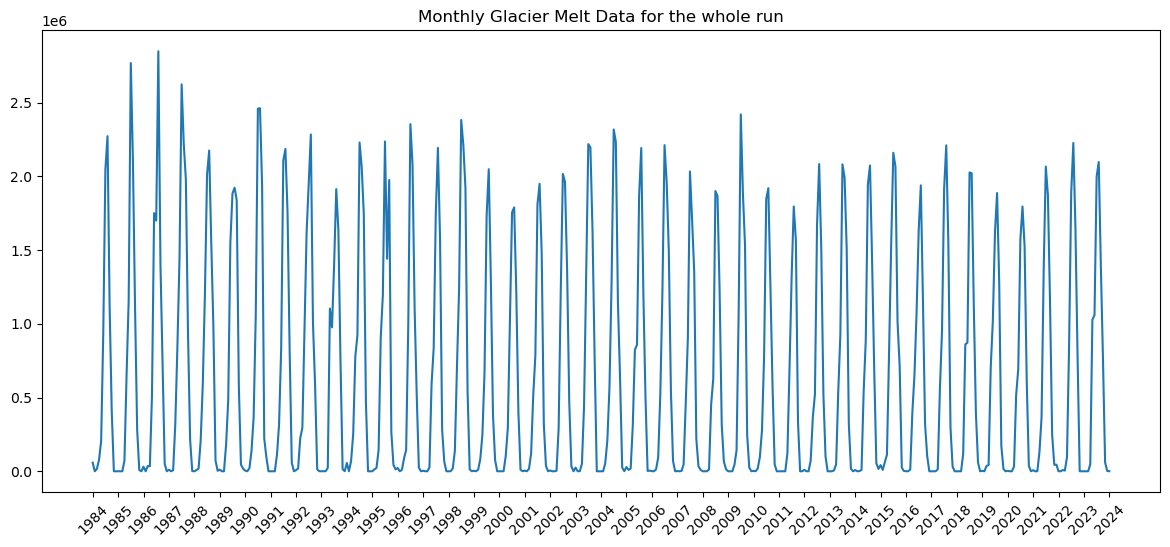
\includegraphics[width=\textwidth]{Plots/glacier_runoff.png}
%         % \caption{Spinup comparison of the model in 1986 after 500 years of spinup and 2 years of run compared with the actual glacier in 1986.}
%         \label{fig:glacier_runoff}
%     \end{subfigure}
%     \hfill
%     \begin{subfigure}[b]{\textwidth}
%         \centering
%         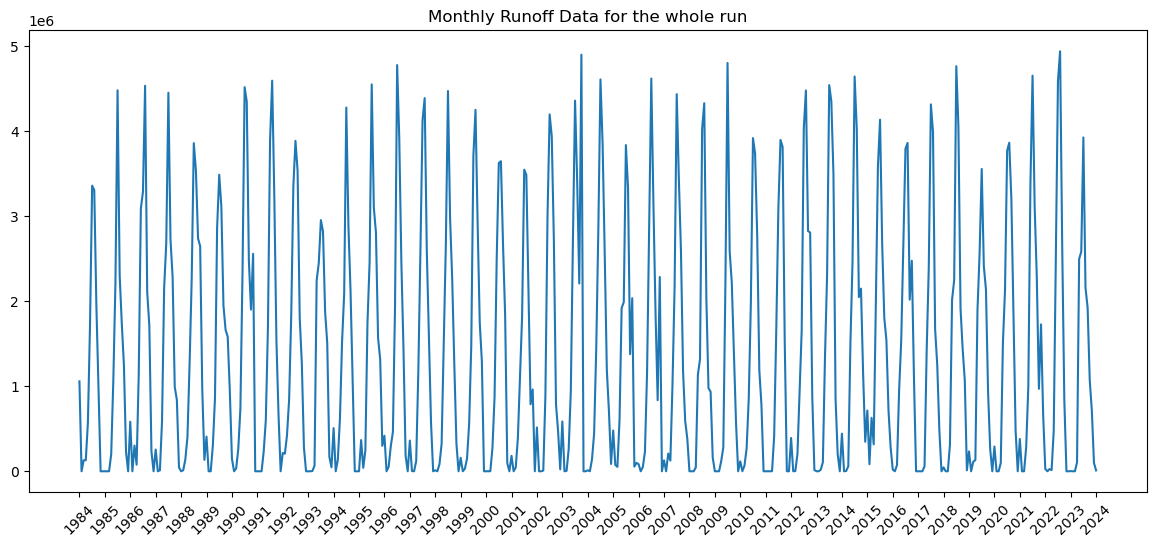
\includegraphics[width=\textwidth]{Plots/all_runoff.png}
%         % \caption{Timing of peak specific runoff as a function of glacier cover.}
%         \label{fig:all_runoff}
%     \end{subfigure}
%     \caption{Comparison plots of the glacier runoff and total basin runoff.}
%     \label{fig:runoff_compare}
% \end{figure}
% \FloatBarrier


% \subsection{What Can Be Improved}
% The largest improvement to this model would be its runtime. It currently takes about 30 seconds to run for 1984-2024, which is most likely 
% due to the use of the Python datetime library which is not very efficient. Eliminating the use of this library would make the model run 
% much faster, but would make it more difficult to run. The datetime library is very useful when using date driven data such as the temperature 
% and precipitation data in this model to keep track of the current date, but it is not very efficient.
\subsection{Future Work}
The next step for this project would be to run the model for a glacier near the South Cascade Glacier with a similar climate to see how region specific the input 
parameters are. Due to the input parameters being tuned for the mass balance of the glacier which largely depends on the local climate, it 
is plausible that they could work well for a glacier with a similar climate.
\paragraph{}
Another idea to explore is to run the model with modeled climate data in order to run the model into the future to see how this glacier 
will evolve and how the basin runoff will evolve.
\textbf{add something about using this model run into the future to see if the earlier peak runoff agrees with  the Fountain and Tangborn 1985 paper and when the peak shifts to}
\section{Conclusion}
\textbf{when i talk about how the model performs better in the long term mention the temperature induced precip error}
The SIA-Mass Balance model is able to model the runoff from the South Cascade Glacier with a RMSE, NSE and KGE of 29.26\%, 0.81 and 0.88 respectively, 
for 16 months from 1992-2007, while the OGGM model errors of 45.96\%, 0.53 and 0.72 for the same time period. This show that complex models are not always 
the best way to model the runoff from small mountain glaciers. A simpler model with parameters tuned to the local climate of the glacier can 
perform just as well, if not better than a more complex model. 
\paragraph{}
From looking at the model error on various time scales, one can see that on longer time scales the SIA-Mass Balance model does quite well. More 
advanced models may be able to model the runoff on shorter timescales with more advanced methods and higher model resolution, but simple models 
like the one used in this study can work well on longer (yearly to decade) timescales.
\paragraph{}
The work of this paper also highlights how important it is to have accurate and reliable weather data for modeling the runoff from glaciers. Inaccurate or 
missing weather data can cause large errors in the model, particularly in the case where the missng data was abnormal.

\begin{thebibliography}{99}

    \bibitem{ref1} Barnett, T.P., J.C. Adam, and D.P. Lettenmaier (2005). **Potential impacts of a warming climate on water availability in snow-dominated regions.** *Nature*, 438(7066), 303–309.
    
    \bibitem{ref2} Milner, A.M., K. Khamis, T.J. Battin, J.E. Brittain, et al. (2017). **Glacier shrinkage driving global changes in downstream systems.** *Proceedings of the National Academy of Sciences (PNAS)*, 114(37), 9770–9778.
    
    \bibitem{ref3} Krimmel, R.M. (1989). **Mass balance and volume of South Cascade Glacier, Washington, 1958–1985.** In J. Oerlemans (Ed.), *Glacier Fluctuations and Climatic Change* (pp. 193–206). Dordrecht: Kluwer Academic Publishers.
    
    \bibitem{ref4} Fountain, A.G., and R.W. Jacobel (1997). **Advances in ice radar studies of a temperate alpine glacier, South Cascade Glacier, Washington, USA.** *Annals of Glaciology*, 24, 303–308.
    
    \bibitem{ref5} ESRI (2011). *ArcGIS Desktop: Release 10*. Redlands, CA: Environmental Systems Research Institute.
    
    \bibitem{ref6} RGI Consortium (2023). **Randolph Glacier Inventory – A Dataset of Global Glacier Outlines: Version 7.0.** Boulder, Colorado, USA: National Snow and Ice Data Center. (doi: 10.5067/F6JMOVY5NAVZ)
    
    \bibitem{ref7} Rasmussen, L.A., and H. Conway (2001). **Estimating South Cascade Glacier (Washington, USA) mass balance from a distant radiosonde and comparison with Blue Glacier.** *Journal of Glaciology*, 47(159), 579–588.
    
    \bibitem{ref8} Harris, C.R., K.J. Millman, S.J. van der Walt, et al. (2020). **Array programming with NumPy.** *Nature*, 585, 357–362.
    
    \bibitem{ref9} O’Neel, S., C. McNeil, L.C. Sass, E. Florentine, et al. (2019). **Reanalysis of the U.S. Geological Survey Benchmark Glaciers: Long-term insight into climate forcing of glacier mass balance.** *Journal of Glaciology*, 65(253), 850–864.
    
    \bibitem{ref10} Virtanen, P., R. Gommers, T.E. Oliphant, et al. (2020). **SciPy 1.0: Fundamental algorithms for scientific computing in Python.** *Nature Methods*, 17(3), 261–272.
    
    \bibitem{ref11} Lange, S., C. Menz, S. Gleixner, M. Cucchi, et al. (2021). **WFDE5 over land merged with ERA5 over the ocean (W5E5 v2.0).** *Earth System Grid Federation (Data Set)*. (doi: 10.48364/ISIMIP.342217)
   
    \bibitem{ref12}Amaral, T., Bartholomaus, T. C., \& Enderlin, E. M. (2020). Evaluation of Iceberg Calving Models Against Observations From Greenland Outlet Glaciers. Journal of Geophysical Research: Earth Surface, 125(6), e2019JF005444. https://doi.org/10.1029/2019JF005444 

    \bibitem{ref13}Auer, I., Böhm, R., Jurkovic, A., Orlik, A., Potzmann, R., Schöner, W., ... \& Zaninovic, K. (2007). HISTALP—historical instrumental climatological surface time series of the Greater Alpine Region. International Journal of Climatology, 27(1), 17-46. DOI: https://doi.org/10.1002/joc.1377. 

    \bibitem{ref14}Brunner, M. I., \& Gilleland, E. (2024). Future changes in floods, droughts, and their extents in the Alps: A sensitivity analysis with a non‐stationary stochastic streamflow generator. Earth's Future, 12, e2023EF004238. https://doi.org/10.1029/2023EF004238 

    \bibitem{ref15}Fountain, A. G., and W. V. Tangborn (1985), The Effect of Glaciers on Streamflow Variations, Water Resour. Res., 21(4), 579–586, doi: https://doi.org/10.1029/WR021i004p00579 

    \bibitem{ref16}GlaThiDa Consortium (2020): Glacier Thickness Database 3.1.0. World Glacier Monitoring Service, Zurich, Switzerland. DOI: https://doi.org/10.5904/wgms-glathida-2020-10 

    \bibitem{ref17}GLIMS Consortium, 2005. GLIMS Glacier Database, Version 1. [Analysis\_IDs 752390--756450, Paul, Frank (submitter); Frey, Holger; Le Bris, Raymond; Paul, Frank; Rastner, Philipp (analyst(s))]. Boulder, Colorado, USA. NASA National Snow and Ice Data Center Distributed Active Archive Center. DOI: https://dx.doi.org/10.7265/N5V98602 

    \bibitem{ref18}Iken, A. (1981). The Effect of the Subglacial Water Pressure on the Sliding Velocity of a Glacier in an Idealized Numerical Model. Journal of Glaciology, 27(97), 407-421. doi: https://doi.org/10.3189/S0022143000011448 

    \bibitem{ref19}Kessler, M. A., Anderson, R. S., \& Stock, G. M. (2006). Modeling topographic and climatic control of east-west asymmetry in Sierra Nevada glacier length during the Last Glacial Maximum. J. Geophys. Res., 111, F02002. doi: https://doi.org/10.1029/2005JF000365. 

    \bibitem{ref20}E. Larour, H. Seroussi, M. Morlighem, and E. Rignot (2012), Continental scale, high order, high spatial resolution, ice sheet modeling using the Ice Sheet System Model, J. Geophys. Res., 117, F01022, doi: https://doi.org/10.1029/2011JF002140 

    \bibitem{ref21}Le Meur, E., Gagliardini, O., Zwinger, T., \& Ruokolainen, J. (2004). Glacier flow modelling: a comparison of the Shallow Ice Approximation and the full-Stokes solution. Comptes Rendus Physique, 5(7), 709-722. https://doi.org/10.1016/j.crhy.2004.10.001. 

    \bibitem{ref22}Naz, B. S., Frans, C. D., Clarke, G. K. C., Burns, P., \& Lettenmaier, D. P. (2014). Modeling the effect of glacier recession on streamflow response using a coupled glacio-hydrological model. Hydrol. Earth Syst. Sci., 18, 787-802. https://doi.org/10.5194/hess-18-787-2014 

    \bibitem{ref23}Paterson, W. S. B. (1994), The Physics of Glaciers, 3rd ed., 481 pp., Else-vier, New York. 

    \bibitem{ref24}Paul, F., Rastner, P., Azzoni, R. S., Diolaiuti, G., Fugazza, D., Le Bris, R., Nemec, J., Rabatel, A., Ramusovic, M., Schwaizer, G., \& Smiraglia, C. (2020). Glacier shrinkage in the Alps continues unabated as revealed by a new glacier inventory from Sentinel-2. Earth Syst. Sci. Data, 12, 1805-1821. https://doi.org/10.5194/essd-12-1805-2020 

    \bibitem{ref25}Verbunt, M., Gurtz, J., Jasper, K., Lang, H., Warmerdam, P., \& Zappa, M. (2003). The hydrological role of snow and glaciers in alpine river basins and their distributed modeling. Journal of Hydrology, 282(1-4), 36-55. https://doi.org/10.1016/S0022-1694(03)00251-8 
\end{thebibliography}
    

\end{document}
